%%
% The BIThesis Template for Bachelor Graduation Thesis
%
% 北京理工大学毕业设计(论文) —— 使用 XeLaTeX 编译
%
% Copyright 2020 Spencer Woo
%
% This work may be distributed and/or modified under the
% conditions of the LaTeX Project Public License, either version 1.3
% of this license or (at your option) any later version.
% The latest version of this license is in
%   http://www.latex-project.org/lppl.txt
% and version 1.3 or later is part of all distributions of LaTeX
% version 2005/12/01 or later.
%
% This work has the LPPL maintenance status `maintained'.
%
% The Current Maintainer of this work is Spencer Woo.
%
% Compile with: xelatex -> biber -> xelatex -> xelatex

% 章节支持、单面打印:ctexbook
\documentclass[UTF8,AutoFakeBold,AutoFakeSlant,zihao=-4,oneside,openany]{ctexbook}
\usepackage[a4paper,left=3cm,right=2.6cm,top=3.5cm,bottom=2.9cm]{geometry}
% 目前 29mm 最接近 Word 排版
\usepackage{xeCJK}
\usepackage{titletoc}
\usepackage{fontspec}
\usepackage{setspace}
\usepackage{graphicx}
\usepackage{fancyhdr}
\usepackage{pdfpages}
\usepackage{setspace}
\usepackage{booktabs}
\usepackage{multirow}
\usepackage{caption}
\usepackage{tikz}
\usetikzlibrary{quotes,angles}
\usepackage{etoolbox}
\usepackage{hyperref}
\usepackage{xcolor}
\usepackage{caption}
\usepackage{array}
\usepackage{bm}
\usepackage{amsmath}
\usepackage{amssymb}
\usepackage{pdfpages}

% 设置参考文献编译后端为 biber,引用格式为 GB/T7714-2015 格式
% 参考文献使用宏包见 https://github.com/hushidong/biblatex-gb7714-2015
\usepackage[
  backend=biber,
  style=gb7714-2015,
  gbalign=gb7714-2015,
  gbnamefmt=lowercase,
  doi=false,
  url=false
]{biblatex}

% 参考文献引用文件位于 misc/ref.bib
\addbibresource{misc/ref.bib}

% 西文字体默认为 Times New Roman
\setromanfont{Times New Roman}
% 论文题目字体为华文细黑
\setCJKfamilyfont{xihei}{STXihei}
\newcommand{\xihei}{\CJKfamily{xihei}}

% 在这里填写你的论文中英文题目
\newcommand{\thesisTitle}{动态跟踪定位问题的算法研究}
\newcommand{\thesisTitleEN}{Algorithm Research of Dynamic Tracking Location Problem}

% 在这里填写你的相关信息
\newcommand{\deptName}{数学与统计学院}
\newcommand{\majorName}{信息与计算科学}
\newcommand{\yourName}{于程洋}
\newcommand{\yourStudentID}{1120170359}
\newcommand{\mentorName}{李庆娜}

% 主题页面格式:BIThesis
\fancypagestyle{BIThesis}{
  % 页眉高度
  \setlength{\headheight}{20pt}
  % 页码高度(不完美,比规定稍微靠下 2mm)
  \setlength{\footskip}{14pt}

  \fancyhf{}
  % 定义页眉、页码
  \fancyhead[C]{\zihao{4}\ziju{0.08}\songti{北京理工大学本科生毕业设计(论文)}}
  \fancyfoot[C]{\songti\zihao{5} \thepage}
  % 页眉分割线稍微粗一些
  \renewcommand{\headrulewidth}{0.6pt}
}

% 设置章节格式
% 一级标题:黑体,三号,加粗;间距:段前 0.5 行,段后 1 行;
\ctexset{chapter={
    name = {第,章},
    number = {\arabic{chapter}},
    format = {\heiti \bfseries \centering \zihao{3}},
    aftername = \hspace{9bp},
    pagestyle = BIThesis,
    beforeskip = 8bp,
    afterskip = 32bp,
    fixskip = true,
  }
}

% 二级标题:黑体,四号,加粗;间距:段前 0.5 行,段后 0 行;
\ctexset{section={
    number = {\thechapter.\hspace{4bp}\arabic{section}},
    format = {\heiti \raggedright \bfseries \zihao{4}},
    aftername = \hspace{8bp},
    beforeskip = 20bp plus 1ex minus .2ex,
    afterskip = 18bp plus .2ex,
    fixskip = true,
  }
}

% 三级标题:黑体、小四、加粗;间距:段前 0.5 行,段后 0 行;
\ctexset{subsection={
    number = {\thechapter.\hspace{3bp}\arabic{section}.\hspace{3bp}\arabic{subsection}},
    format = {\heiti \bfseries \raggedright \zihao{-4}},
    aftername = \hspace{7bp},
    beforeskip = 17bp plus 1ex minus .2ex,
    afterskip = 14bp plus .2ex,
    fixskip = true,
  }
}

% 设置目录样式
% 添加 PDF 链接
\addtocontents{toc}{\protect\hypersetup{hidelinks}}

% 解决「目录」二字的格式问题
\renewcommand{\contentsname}{
  \fontsize{16pt}{\baselineskip}
  \normalfont\heiti{目~~~~录}
  \vspace{-8pt}
}
% 定义目录样式
\titlecontents{chapter}[0pt]{\songti \zihao{-4}}
{\thecontentslabel\hspace{\ccwd}}{}
{\hspace{.5em}\titlerule*{.}\contentspage}
\titlecontents{section}[2\ccwd]{\songti \zihao{-4}}
{\thecontentslabel\hspace{\ccwd}}{}
{\hspace{.5em}\titlerule*{.}\contentspage}
\titlecontents{subsection}[4\ccwd]{\songti \zihao{-4}}
{\thecontentslabel\hspace{\ccwd}}{}
{\hspace{.5em}\titlerule*{.}\contentspage}

% 前置页面(原创性声明、中英文摘要、目录等)
\renewcommand{\frontmatter}{
  \pagenumbering{Roman}
  \pagestyle{BIThesis}
}

% 正文页面
\renewcommand{\mainmatter}{
  \pagenumbering{arabic}
  \pagestyle{BIThesis}
}

% 设置 caption 与 figure 之间的距离
\setlength{\abovecaptionskip}{11pt}
\setlength{\belowcaptionskip}{9pt}

% 设置图片的 caption 格式
\renewcommand{\thefigure}{\thechapter-\arabic{figure}}
\captionsetup[figure]{font=small,labelsep=space}

% 设置表格的 caption 与 table 之间的垂直距离
\captionsetup[table]{skip=2pt}

% 设置表格的 caption 格式
\renewcommand{\thetable}{\thechapter-\arabic{table}}
\captionsetup[table]{font=small,labelsep=space}

% 设置数学公式编号格式
\renewcommand{\theequation}{\arabic{chapter}-\arabic{equation}}

% 文档开始
\begin{document}

% 标题页面:如无特殊需要,本部分无需改动
%%
% The BIThesis Template for Bachelor Graduation Thesis
%
% 北京理工大学毕业设计(论文)封面页 —— 使用 XeLaTeX 编译
%
% Copyright 2020 Spencer Woo
%
% This work may be distributed and/or modified under the
% conditions of the LaTeX Project Public License, either version 1.3
% of this license or (at your option) any later version.
% The latest version of this license is in
%   http://www.latex-project.org/lppl.txt
% and version 1.3 or later is part of all distributions of LaTeX
% version 2005/12/01 or later.
%
% This work has the LPPL maintenance status `maintained'.
%
% The Current Maintainer of this work is Spencer Woo.
%
% 封面
%
% 如无特殊需要,本页面无需更改

% Underline new command for student information
% Usage: \dunderline[<offset>]{<line_thickness>}
\newcommand\dunderline[3][-1pt]{{%
  \setbox0=\hbox{#3}
  \ooalign{\copy0\cr\rule[\dimexpr#1-#2\relax]{\wd0}{#2}}}}

% Cover Page
\begin{titlepage}
  \vspace*{19mm}
  \centering

  
\includegraphics[width=9.87cm]{images/header.png}

  \vspace*{-3mm}

  \zihao{-0}\textbf{\ziju{0.12}\songti{本科生毕业设计(论文)}}

  \vspace{16mm}

  \zihao{2}\textbf{\xihei\thesisTitle}

  \vspace{3mm}

  \begin{spacing}{1.2}
    \zihao{3}\selectfont{\textbf{\thesisTitleEN}}
  \end{spacing}

  \vspace{15mm}

  \flushleft
  \begin{spacing}{1.8}
    \hspace{27mm}\songti\zihao{3}\selectfont{学\hspace{11mm}院:\dunderline[-10pt]{1pt}{\makebox[78mm][c]{\deptName}}}

    \hspace{27mm}\songti\zihao{3}\selectfont{专\hspace{11mm}业:\dunderline[-10pt]{1pt}{\makebox[78mm][c]{\majorName}}}

    \hspace{27mm}\songti\zihao{3}\selectfont{学生姓名:\dunderline[-10pt]{1pt}{\makebox[78mm][c]{\yourName}}}

    \hspace{27mm}\songti\zihao{3}\selectfont{学\hspace{11mm}号:\dunderline[-10pt]{1pt}{\makebox[78mm][c]{\yourStudentID}}}

    \hspace{27mm}\songti\zihao{3}\selectfont{指导教师:\dunderline[-10pt]{1pt}{\makebox[78mm][c]{\mentorName}}}
  \end{spacing}

  \vspace{25mm}

  \centering
  \zihao{3}\ziju{0.5}\songti{\today}
\end{titlepage}


% 前置页面定义
\frontmatter
% 原创性声明:如无特殊需要,本部分无需改动
% 更改为 PDF 页面插入,如需要添加内容,可考虑先用 Word 制作再覆盖 misc/1_originality.pdf

\includepdf{misc/1_originality.pdf}
\newpage
%%%
% The BIThesis Template for Bachelor Graduation Thesis
%
% 北京理工大学毕业设计(论文)原创性声明页 —— 使用 XeLaTeX 编译
%
% Copyright 2020 Spencer Woo
%
% This work may be distributed and/or modified under the
% conditions of the LaTeX Project Public License, either version 1.3
% of this license or (at your option) any later version.
% The latest version of this license is in
%   http://www.latex-project.org/lppl.txt
% and version 1.3 or later is part of all distributions of LaTeX
% version 2005/12/01 or later.
%
% This work has the LPPL maintenance status `maintained'.
%
% The Current Maintainer of this work is Spencer Woo.
%
% 如无特殊需要,本页面无需更改

% 原创性声明页无页码页面格式
\fancypagestyle{originality}{
  % 页眉高度
  \setlength{\headheight}{20pt}

  % 页眉和页脚(页码)的格式设定
  \fancyhf{}
  \fancyhead[C]{\zihao{4}\ziju{0.08}\songti{北京理工大学本科生毕业设计(论文)}}

  % 页眉分割线稍微粗一些
  \renewcommand{\headrulewidth}{0.6pt}
}

\pagestyle{originality}
\topskip=0pt

% 圆形数字编号定义
\newcommand{\circled}[2][]{\tikz[baseline=(char.base)]
  {\node[shape = circle, draw, inner sep = 1pt]
  (char) {\phantom{\ifblank{#1}{#2}{#1}}};
  \node at (char.center) {\makebox[0pt][c]{#2}};}}
\robustify{\circled}

% 设置行间距
\setlength{\parskip}{0.4em}
\renewcommand{\baselinestretch}{1.41}

% 顶部空白
\vspace*{-6mm}

% 原创性声明部分
\begin{center}
  \heiti\zihao{2}\textbf{原创性声明}
\end{center}

% 本部分字号为小三
\zihao{-3}

本人郑重声明:所呈交的毕业设计(论文),是本人在指导老师的指导下独立进行研究所取得的成果。除文中已经注明引用的内容外,本文不包含任何其他个人或集体已经发表或撰写过的研究成果。对本文的研究做出重要贡献的个人和集体,均已在文中以明确方式标明。

特此申明。

\vspace{13mm}

\begin{flushright}
  本人签名:\hspace{40mm}日\hspace{2.5mm}期:\hspace{13mm}年\hspace{8mm}月\hspace{8mm}日
\end{flushright}

\vspace{17mm}

% 使用授权声明部分
\begin{center}
  \heiti\zihao{2}\textbf{关于使用授权的声明}
\end{center}

本人完全了解北京理工大学有关保管、使用毕业设计(论文)的规定,其中包括:\circled{1}学校有权保管、并向有关部门送交本毕业设计(论文)的原件与复印件;\circled{2}学校可以采用影印、缩印或其它复制手段复制并保存本毕业设计(论文);\circled{3}学校可允许本毕业设计(论文)被查阅或借阅;\circled{4}学校可以学术交流为目的,复制赠送和交换本毕业设计(论文);\circled{5}学校可以公布本毕业设计(论文)的全部或部分内容。

\vspace*{1mm}

\begin{flushright}
  \begin{spacing}{1.65}
    \zihao{-3}
    本人签名:\hspace{40mm}日\hspace{2.5mm}期:\hspace{13mm}年\hspace{8mm}月\hspace{8mm}日\\
    指导老师签名:\hspace{40mm}日\hspace{2.5mm}期:\hspace{13mm}年\hspace{8mm}月\hspace{8mm}日
  \end{spacing}
\end{flushright}

\newpage

% 摘要:在摘要相应的 TeX 文件处进行摘要部分的撰写
%%
% The BIThesis Template for Bachelor Graduation Thesis
%
% 北京理工大学毕业设计(论文)中英文摘要 —— 使用 XeLaTeX 编译
%
% Copyright 2020 Spencer Woo
%
% This work may be distributed and/or modified under the
% conditions of the LaTeX Project Public License, either version 1.3
% of this license or (at your option) any later version.
% The latest version of this license is in
%   http://www.latex-project.org/lppl.txt
% and version 1.3 or later is part of all distributions of LaTeX
% version 2005/12/01 or later.
%
% This work has the LPPL maintenance status `maintained'.
%
% The Current Maintainer of this work is Spencer Woo.

% 中英文摘要章节
\topskip=0pt
\zihao{-4}

\vspace*{-7mm}

\begin{center}
  \heiti\zihao{-2}\textbf{\thesisTitle}
\end{center}

\vspace*{2mm}

\addcontentsline{toc}{chapter}{摘~~~~要}
{\let\clearpage\relax \chapter*{\textmd{摘~~~~要}}}
\setcounter{page}{1}

\vspace*{1mm}

\setstretch{1.53}
\setlength{\parskip}{0em}

% 中文摘要正文从这里开始
单站无源跟踪定位是一项重要的定位技术,可以补充多站跟踪定位在灵活性方面的不足,但是单站定位通常得到得观测量数据比多站定位少,因此定位难度较高。本文主要研究基于纯角度的单站无源跟踪定位算法,利用测向定位法的原理实现对目标的定位跟踪。但是在观测站运动的过程中方位角和仰角的变化幅度很小,容易受到噪声的影响,导致定位误差较大。本文考虑普通最小二乘法(OLS)、总体最小二乘法(TLS)、极大似然估计法(MLE)、渐进无偏估计(AUE)四种算法对模型进行求解。比较算法的性能,并探究影响定位结果的因素。最终得出AUE算法是精确度最好的一种算法,并且得到当目标与观测站的距离越近,定位的精确度越高。方位角和仰角做为影响定位结果的两种重要因素,变化幅度越大,定位的精确度越高。

\vspace{4ex}\noindent\textbf{\heiti 关键词:单站无源跟踪定位,测向定位,OLS,TLS,MLE,AUE}
\newpage

% 英文摘要章节
\topskip=0pt

\vspace*{2mm}

\begin{spacing}{0.95}
  \centering
  \heiti\zihao{3}\textbf{\thesisTitleEN}
\end{spacing}

\vspace*{17mm}

\addcontentsline{toc}{chapter}{Abstract}
{\let\clearpage\relax \chapter*{
  \zihao{-3}\textmd{Abstract}\vskip -3bp}}
\setcounter{page}{2}

\setstretch{1.53}
\setlength{\parskip}{0em}

% 英文摘要正文从这里开始
Single-station passive tracking and positioning is an important positioning technology that can supply the flexibility of multi-station tracking and positioning, but single-station positioning usually obtains less observational data than multi-station positioning, so single-station positioning is more difficult. This paper mainly studies the single-station passive tracking and positioning algorithms based on bearing-only, using the principle of directional cosine intersection positioning method to achieve the tracking and positioning of target. however, the azimuth and elevation angles change very little during the movement of observation station, which is susceptible to the influence of noise, leading to large positioning errors. This paper considers four algorithms, Ordinary Least Squares(OLS), Total Least Squares(TLS), Maximum Likelihood Estimation(MLE), and Approximate Unbiased Estimation(AUE), to solve the model. Comparing the performance of the algorithms and exploring the factors that affect the positioning results. It is concluded that the AUE algorithm is the one with the best accuracy, and it is obtained that the closer the distance between the target and the observing station, the higher the positioning accuracy.  Azimuth angle and elevation angle are two important factors that affect the positioning result. The bigger the range of change, the higher the accuracy of positioning results.

\vspace{3ex}\noindent\textbf{Key Words: Single-station Passive Tracking Positioning,Directional Cosine Intersection Positioning,OLS,TLS,MLE,AUE}
\newpage

% 目录:如无特殊需要,本部分无需改动
%%
% The BIThesis Template for Bachelor Graduation Thesis
%
% 北京理工大学毕业设计(论文)目录 —— 使用 XeLaTeX 编译
%
% Copyright 2020 Spencer Woo
%
% This work may be distributed and/or modified under the
% conditions of the LaTeX Project Public License, either version 1.3
% of this license or (at your option) any later version.
% The latest version of this license is in
%   http://www.latex-project.org/lppl.txt
% and version 1.3 or later is part of all distributions of LaTeX
% version 2005/12/01 or later.
%
% This work has the LPPL maintenance status `maintained'.
%
% The Current Maintainer of this work is Spencer Woo.
%
% 如无特殊需要,本页面无需更改

% 目录开始

% 调整目录行间距
\renewcommand{\baselinestretch}{1.35}
% 目录
\tableofcontents
\newpage


% 正文开始
\mainmatter
% 正文 22 磅的行距
\setlength{\parskip}{0em}
\renewcommand{\baselinestretch}{1.53}

% 第一章
%%
% The BIThesis Template for Bachelor Graduation Thesis
%
% 北京理工大学毕业设计(论文)第一章节 —— 使用 XeLaTeX 编译
%
% Copyright 2020 Spencer Woo
%
% This work may be distributed and/or modified under the
% conditions of the LaTeX Project Public License, either version 1.3
% of this license or (at your option) any later version.
% The latest version of this license is in
%   http://www.latex-project.org/lppl.txt
% and version 1.3 or later is part of all distributions of LaTeX
% version 2005/12/01 or later.
%
% This work has the LPPL maintenance status `maintained'.
%
% The Current Maintainer of this work is Spencer Woo.
%
% 第一章节

\chapter{引言}

\section{跟踪定位背景介绍}
定位技术在现代社会中被广泛应用,对人们的日常生活、勘探作业以及国防事业等都具有重要意义。随着定位技术的发展也产生了不同方式的定位技术,如无线传感网络(WSN)定位技术\cite{wls1}\cite{wls2}\cite{wsl3}\cite{wsl4},通过多个传感器组成的无线通信网络在其监控的区域内实现目标的定位,可以应用于事件检测(火灾、洪水、冰雹),监视(工业,农业)等,定位算法也比较完善。水声定位系统\cite{bls5}\cite{bls6}\cite{bls7}\cite{bls8},利用水声探测装置通过测量声源到基元之间的相关信息量实现对声源的定位,根据定位系统的基阵长度可以分为:长基线、短基线和超短基线,通常用于对水下目标的勘察。

除此之外,无源定位与跟踪定位技术在国防事业上的应用具有更为重要的意义\cite{9},按照不同定位方法进行划分,无源定位可以分为基于测向的测角定位法、基于测信号到达时间差的时差定位法、基于相对运动产生多普勒频率的频率定位方法,以及这些方法的混合方法。按照定位系统的观测站数量又可划分为单站定位和多站定位。一方面,由于多站定位会存在站间通信稳定、站间信号匹配等方面的问题,而单站定位有着较强的机动性和适应性,另一方面,在固定多站或运动多站的设备受到影响时,定位结果也会受到影响,此时单站定位可以作为补充手段。因此,单站无源定位与跟踪技术的发展显得尤为重要
\section{测向定位法(BO)及算法简述}
单站无源定位跟踪技术是利用一个观测站对目标进行无源定位的技术,由于获得的信息量相对较少,所以实现定位的难度相对较大。在定位时,由观测站对目标进行连续的测量,在获得一定的定位信息后,经过适当的数据处理获得目标的定位信息。

单站跟踪定位在很多应用场合目标是运动的,对于固定的目标观测站可通过连续的运动获得目标的角度信息,再通过三角定位法对其定位,该问题相对简单。本文考虑的场景为运动的目标,根据文献\cite{10}的第8章,利用对运动的目标的测量信息有可能获得目标位置和运动状态的过程称为目标运动分析(Target Motion Analysis,TMA)。按照观测其的运动方式,TMA可分为两类,第一类观测站自身是机动的,第二类观测站无机动运动。对两类观测站应用不同的跟踪定位方法可能会得到不同的定位结果。目前,单站无源跟踪定位技术采用的方法主要有\cite{11}:到达时间定位法(TOA)、多普勒频率定位法、测向定位法(BO),以及联合信息定位法。然而对于运动的目标只测量单一的信息量通常并不能得到目标的全部运动状态,通常需要联合两种或多种信息量以实现对目标的测量。不过对观测站的运动状态做相应的要求也可以实现对特殊运动状态的目标进行定位跟踪。其中测向定位法的研究较为完善。

测向定位法是单站无源跟踪定位技术中研究最多最主要的一种方法,测向定位法是指仅利用目标相对于观测站的角度信息对目标进行定位。当观测站固定时,文献\cite{10}中8.4节指出对于二维平面上匀速直线运动的目标,只要其运动方向不是径向的,就可以通过三次以上的测量确定目标的运动方向,但是不能得到目标的距离及速度大小。文献\cite{12}在测角信息的基础上添加径向加速度信息,得出对于非径向运动的匀速运动目标,利用径向加速度信息和角度信息可以实现对目标的定位,并且目标距离越近,相对运动速率越大运动方向越接近切向,其可观测度越高,并且由于观测站与目标轨迹可构成二维平面,故该结论可以推到三维空间。

对于运动的观测站,实质是利用多次观测来拟合目标的运动轨迹,文献\cite{bo1}\cite{bo2}给出了目标可观测性条件,其中文献\cite{bo1}给出了二维平面上匀速直线运动目标可观测的充要条件,文献\cite{bo2}给出了三维空间上匀速直线运动目标可观测的充要条件。因此对于满足条件的机动观测站可实现对匀速目标的定位跟踪。

对于纯角度单站无源跟踪定位的算法主要有最小二乘法(LS)、极大似然估计法(MLE)、、近似无偏估计法(AUE)以及卡尔曼滤波法(KF)。文献\cite{15},\cite{wls2}通过对角度信息量的处理,将非线性的测量方程转化为线性方程求解,由此得到了处理角度信息的最小二乘法。文献\cite{16}推导了二维平面上匀速目标基于奇异值分解(SVD)的总体最小二乘法。文献\cite{15}通过对角度信息的噪声概率密度函数分析得到其极大似然估计函数,并在考虑加权对位置定位的影响时得到了极大似然估计的迭代算法。文献\cite{10}中第9章中推导了二维平面上基于纯角度信息对匀速运动目标进行定位的极大似然估计的迭代算法。由于在考虑噪声误差的情况下,最小二乘法是有偏估计,文献\cite{17}提出了二维平面上基于角度的双站无源定位近似无偏估计,与扩展卡尔曼滤波法相比,该方法的收敛速度和误差精度都相对较好。文献\cite{18}提出了基于角度和时差的双站定位的近似无偏估计算法,结果表明与有偏估计算法相比该算法具有更高的精度。文献\cite{19}给出了卡尔曼滤波和扩展卡尔曼滤波的方法和原理,卡尔曼滤波对模型线性的要求较高,无法直接应用于非线性无源定位系统。通过对卡尔曼滤波加以扩展和改进可以得到适应于非线性模型的无源定位系统,扩展卡尔曼滤波(EKF)即可用于解决非线性的无源定位模型。不过在将非线性模型线性化的过程中通常会带来误差,导致收敛不稳定,甚至发散,使其应用受限。文献\cite{20}基于扩展卡尔曼滤波提出了一种改进算法,该算法可以消除不利误差的影响,并提高定位精度。不过卡尔曼滤波算法计算量相对较大,并且对迭代初值的依赖较大,通常会出现不收敛的情况。

本文研究的问题是基于纯角度的单站跟踪定位算法,并根据上述相关文献推导了三维空间上基于纯角度的匀速运动目标的跟踪定位的相关算法,包括最小二乘法、总体最小二乘法、极大似然估计法和近似无偏估计法。最后通过数值实验比较四种算法的性能。

%%
% The BIThesis Template for Bachelor Graduation Thesis
%
% 北京理工大学毕业设计(论文)第一章节 —— 使用 XeLaTeX 编译
%
% Copyright 2020 Spencer Woo
%
% This work may be distributed and/or modified under the
% conditions of the LaTeX Project Public License, either version 1.3
% of this license or (at your option) any later version.
% The latest version of this license is in
%   http://www.latex-project.org/lppl.txt
% and version 1.3 or later is part of all distributions of LaTeX
% version 2005/12/01 or later.
%
% This work has the LPPL maintenance status `maintained'.
%
% The Current Maintainer of this work is Spencer Woo.
%
% 第一章节

\chapter{基于纯角度信息的单站跟踪定位模型}
本文主要讨论三维空间中基于纯角度信息的单站无源跟踪定位问题,关于该问题的模型如下图所示:

\begin{figure}[h]
  \vspace{13pt}
  \centering
  \begin{tikzpicture}[scale=0.66]
      \draw[->] (0,0) -- (13,0) node[below] {$X$};
      \draw[->] (0,0) -- (5,6.67) node[left] {$Y$};
      \draw[->] (0,0) -- (0,10) node[left] {$Z$};
      \draw (0,0) node[below] {$O$};
      \draw[->] (3,1) node[below] {$B$} -- (4,0.8) node[below] {$\bm{v_B}$};
      \draw[->] (9,6) node[left] {$G$} -- (10,6.3) node[above] {$\bm{v_G}$};
      \draw[dashed] (9,6) -- (9,3);
      \coordinate (a) at (7.5,1);
      \coordinate (b) at (3,1);
      \coordinate (c) at (9,3);
      \coordinate (d) at (9,6);
      \draw[dashed] (a) -- (b) -- (c)
        pic [draw, ->, "$\scriptstyle\beta$", angle radius=7mm, angle eccentricity=1.5] {angle = a--b--c};
      \draw[dashed] (c) -- (b) -- (d) 
        pic [draw, ->, "$\varepsilon$", angle radius=5mm, angle eccentricity=1.5] {angle = c--b--d};
     
      \draw (b) -- (d);
      \draw[dashed] (9,1) -- (a);
      \draw[dashed] (1,1) -- (b);
  \end{tikzpicture}
  \caption{纯角度单站跟踪定位模型示意图}
\end{figure}

其中,$G$ 表示运动的目标,$B$ 表示运动的观测站,$\bm{v_G}$ 和 $\bm{v_B}$ 分别表示目标和观测站运动的速度矢量,$\varepsilon$ 表示目标 $G$ 和观测站 $B$ 连线与 $XOY$ 平面形成的夹角,并称之为仰角,$\beta$ 表示目标 $G$ 在 $XOY$ 平面的投影点和观测站 $B$ 连线与 $X$ 轴正向形成的夹角,并称之为方位角。

在纯角度信息的单站跟踪定位模型中,观测站的运动信息是已知的,观测站每经过时间 $T$ 对运动的目标进行一次测量,得到目标的仰角和方位角测量值,然后根据这些已知信息对目标进行定位跟踪。然而,在多数情况下,单站无源定位在仅有角度信息时只能描述目标所在的方向,无法确定目标的距离,从而也就无法确定目标的实际位置。因此需要对运动目标的可观测性进行分析。
\section{可观测性分析}
假设目标做匀速直线运动,根据文献\cite{4104040},假设目标 $G$ 的位置坐标为 $(r_{Gx},r_{Gy},r_{Gz})$,以速度 $(v_{Gx},v_{Gy},v_{Gz})$ 匀速运动,故目标在坐标系下的状态矢量可表示为 
\begin{equation*}
	\bm{X}_{G} = [r_{Gx},r_{Gy},r_{Gz},v_{Gx},v_{Gy},v_{Gz}]^T
\end{equation*} 
同样的,观测站的状态矢量可表示为 
\begin{equation*}
	\bm{X}_B = [r_{Bx},r_{By},r_{Bz},v_{Bx},v_{By},v_{Bz}]^T
\end{equation*}
则目标相对于观测站的状态矢量可表示为
\begin{equation}
	\bm{X} = \bm{X}_G - \bm{X}_B = [r_x,r_y,r_z,v_x,v_y,v_z]^T
\end{equation}
从而得到
\begin{equation}
	\dot{\bm{X}} = A\bm{X} - \bm{u} \label{eq:1}
\end{equation}
其中
\begin{equation*}
		A = \left[ \begin{array}{ccc|ccc}
			0 & 0 & 0 & 1 & 0 & 0 \\
			0 & 0 & 0 & 0 & 1 & 0 \\
			0 & 0 & 0 & 0 & 0 & 1 \\ \hline 
			0 & 0 & 0 & 0 & 0 & 0 \\
			0 & 0 & 0 & 0 & 0 & 0 \\
			0 & 0 & 0 & 0 & 0 & 0 \\
		\end{array} \right ], \quad
	\bm{u} = [\bm{0}, \bm{a}^T ]^T = [0, 0, 0, a_x, a_y, a_z]^T 
\end{equation*}
$\bm{a} = [a_x,a_y,a_z]^T$ 表示观测站的加速度,对式\ref{eq:1}求积分可得
\begin{equation}
	\begin{split}
		\bm{r}(t) =& \bm{r}(t_0) + (t-t_0)\bm{v}(t_0) - \int_{t_0}^{t}(t-\tau)\bm{a}(\tau)d\tau \\
		\bm{v}(t) =& \bm{v}(t_0) - \int_{t_0}^{t}\bm{a}(\tau)d\tau
	\end{split}	
\end{equation}
其中 $t_0$ 表示任意确定的初始时刻。

对于方位角和仰角,根据几何知识可以得到
\begin{equation}
	\begin{split}
		\beta =& \arctan \frac{r_y}{r_x} \\
		\varepsilon =& \arctan \frac{r_z}{\sqrt{r_x^2 + r_y^2}}
	\end{split}
\end{equation}
对上式做等价变形可得到(参见附录中A部分)
\begin{equation}
	H\bm{X}=\bm{0} \label{eq:2}
\end{equation}
其中
\begin{equation*}
	H = \left[\begin{array}{cccccc}
		1 & 0 & -\cos\beta\cot\varepsilon & 0 & 0 & 0\\
		0 & 1 & -\sin\beta\cot\varepsilon & 0 & 0 & 0
	\end{array}\right]
\end{equation*}
假定 $\varepsilon \not \equiv 0$,在不考虑噪声的情况下,可以精确确定 $\bm{H}$,根据附录中B部分结论可对式(\ref{eq:1})和式(\ref{eq:2})的线性系统进行处理,从而得到可观测性的充分必要条件,即目标可被唯一确定的充分必要条件。
\begin{equation}
	\det[C^TC] \not \equiv 0
\end{equation}
其中
\begin{equation}
	C = \left[\begin{array}{c}
		C_0 \\ \hline
		C_1 \\ \hline
		C_2 \\ \hline
		C_3 \\ \hline
		C_4 \\ \hline
		C_5 
	\end{array}\right] 
	= \left[\begin{array}{c}
		H \\ \hline
		\dot{C_0} + C_0 A \\ \hline
		\dot{C_1} + C_1 A \\ \hline
		\dot{C_2} + C_2 A \\ \hline
		\dot{C_3} + C_3 A \\ \hline
		\dot{C_4} + C_4 A 
	\end{array}\right]
\end{equation}
由于 $A$ 和 $H$ 都是稀疏矩阵,可以得到 $C$ 的形式如下
\begin{equation}
	C = \left[\begin{array}{c|c|c|c}
		I & \bm{h}_0 & O & \bm{0} \\ \hline
		O & \bm{h}_1 & I & \bm{h}_0 \\ \hline
		O & \bm{h}_2 & O & 2\bm{h}_1 \\ \hline
		O & \bm{h}_3 & O & 3\bm{h}_2 \\ \hline
		O & \bm{h}_4 & O & 4\bm{h}_3 \\ \hline
		O & \bm{h}_5 & O & 5\bm{h}_4
	\end{array}\right]
\end{equation}
其中,$I$ 是 $2 \times 2$ 的单位矩阵,$O$ 是 $2 \times 2$ 的零矩阵,并且有
\begin{equation}
	\bm{h}_i = \left[\begin{array}{c}
		f_i \\ g_i
	\end{array}\right] = - \left[\begin{array}{c}
	\frac{d^i(\cos\beta\cot\varepsilon)}{dt^i} \\
	\frac{d^i(\sin\beta\cot\varepsilon)}{dt^i}
\end{array}\right] \quad i=0,1,2,\cdots
\end{equation}
将矩阵 $C$ 的第二个和第三个分区列互换,此时 $\det[C^TC]$ 的值并不会改变,在结合行列式简化公式(参见附录中C部分)可得到
\begin{equation}
	\det[C^TC] = \det \left[\begin{array}{cc}
		\sum_{i=1}^{4}\bm{h}'_{i+1}\bm{h}_{i+1} & \sum_{i=1}^{4}(i+1)\bm{h}'_{i+1}\bm{h}_i \\
		\sum_{i=1}^{4} (i+1)\bm{h}'_{i}\bm{h}_{i+1} & \sum_{i=1}^{4}(i+1)^2\bm{h}'_i\bm{h}_i
	\end{array}\right]
\end{equation}
最终得到
\begin{equation}
	\begin{split}
		\det[C^TC] =& \frac{1}{2}\sum_{i=1}^{4}\sum_{j=1}^{4}\lbrace [(i+1)f_i f_{j+1} - (j+1)f_j f_{i+1}]^2 + 2[(i+1)f_i g_{j+1} - (j+1) g_j f_{i+1}]^2 \\
		&+ [(i+1)g_i g_{j+1} - (j+1)g_j g_{i+1}]^2 \rbrace
	\end{split}	\label{eq:3}
\end{equation}
由式(\ref{eq:3})可看出,当且仅当两次求和中至少有一项不完全相同时,才满足 $\det[C^TC] \not \equiv 0$,根据附录中C部分可以得到满足该条件的充分必要条件为
\begin{equation}
	\int_{t_0}^{t}(t-\tau)\bm{a}(\tau)d\tau \not \equiv \alpha(t)[\bm{r}(t_0)+(t-t_0)\bm{v}(t_0)]
\end{equation}
对任意的标量函数 $\alpha$ 成立

通过以上描述,得到了目标做匀速直线运动时的可观测性条件。本文的以下内容是在可观测的条件下对纯角度的单站无源定位模型进行分析求解。
\section{跟踪定位模型}
假设目标做匀速直线运动,在 $k$ 个时间周期,每个时间周期时间为 $T$,观测站从初始时刻(记初始时刻 $t_0=0$)开始测量目标的方位信息,之后每经过时间周期 $T$ 对目标的方位信息进行一次测量,得到目标相对于观测站的仰角和方位角分别为 $\varepsilon_i$ 和 $\beta_i$,其中 $k = 0,1,2,\cdots,k$ 

根据图(2-1)及几何关系可得:
\begin{equation}
	\begin{cases}
		\beta_i = \arctan \frac{y_i-B_{iy}}{x_i-B_{ix}} &i=0,1,2,\cdots,k \\
		\varepsilon_i = \arctan \frac{z_i-B_{iz}}{\sqrt{(x_i-B_{ix})^2 + (y_i - B_{iy})^2}} \quad &i=0,1,2,\cdots,k
	\end{cases}\label{eq:arctan}
\end{equation}
其中,$(B_{ix},B_{iy},B_{iz})$ 表示观测站 $B$ 在时刻 $iT$ 时的坐标,$\bm{X}_i = (x_i,y_i,z_i,v_x,v_y,v_z)^T$ 表示目标在时刻 $iT$ 时的状态矢量,从而可以由目标在 $iT$ 时刻的状态得到目标在 $jT$ 时刻的状态:
\begin{equation}
	\begin{cases}
		x_j = x_i + v_x(j-i)T\\
		y_j = y_i + v_y (j-i)T\\
		z_j = z_i + v_z(j-i)T
	\end{cases}
\end{equation}
其中 $i,j \in \lbrace 0,1,2,\cdots,k \rbrace$。根据三角函数公式并结合式(2-14)可以对式(\ref{eq:arctan})进行如下变形:
\begin{equation}
	\begin{cases}
		\cos\beta_i(y_j + v_y(i-j)T-B_{iy}) = \sin\beta_i(x_j+v_x(i-j)T-B_{ix}) \\
		\sin\varepsilon_i \cos\beta_i(x_j+v_x(i-j)T-B_{ix}) + \sin\varepsilon_i \sin\beta_i(y_j + v_y(i-j)T-B_{iy}) \\
		 = \cos\varepsilon_i (z_j + v_z(i-j)T - B_{iz})
	\end{cases}
\end{equation}
其中 $i=0,1,2,\cdots,k,j \in \lbrace 0,1,2,\cdots,k \rbrace$。
由于在实际情况中测量角度得到的观测值可能存在噪声,并不是真实值,即
\begin{equation}
	\begin{cases}
		\beta_{mi} = \beta_i + n_{\beta i} \\
		\varepsilon_{mi} = \varepsilon_i + n_{\varepsilon i}
	\end{cases}
\end{equation}
其中,$\beta_{mi},\varepsilon_{mi}$ 表示观测值,$\beta_i,\varepsilon_i$ 表示真实值,$n_{\beta i},n_{\varepsilon i}$ 表示误差值,并假设 $n_{\beta i} \sim N(0,\sigma^2),n_{\varepsilon i} \sim N(0,\sigma^2)$,且$n_{\beta i},n_{\varepsilon i}$相互独立。
由 Taylor 展开,令$n_{\varepsilon i} \rightarrow 0,n_{\beta i} \rightarrow 0$,可以得到
\begin{equation}
	\begin{cases}
		\cos\beta_i = \cos\beta_{mi} + \sin\beta_{mi}n_{\beta i} + o(n_{\beta i}) \\
		\sin\beta_i = \sin\beta_{mi} - \cos\beta_{mi}n_{\beta i} + o(n_{\beta i}) \\
		\cos\varepsilon_i = \cos\varepsilon_{mi} + \sin\varepsilon_{mi}n_{\varepsilon i} + o(n_{\varepsilon i}) \\
		\sin\varepsilon_i = \sin\varepsilon_{mi} - \cos\varepsilon_{mi}n_{\varepsilon i} + o(n_{\varepsilon i})
	\end{cases}
\end{equation}
当 $n_{\varepsilon i}\rightarrow 0 , n_{\beta i} \rightarrow 0$ 时,可得 $o(n_{\beta i}) \approx 0, o(n_{\varepsilon i}) \approx 0, n_{\beta i}n_{\varepsilon i} \approx 0$,对这些无穷小量忽略不计,可将式(2-15)改写为
\begin{equation}
	\begin{cases}
		-(\sin\beta_{mi} - \cos\beta_{mi}n_{\beta i})x_j +(\cos\beta_{mi} + \sin\beta_{mi}n_{\beta i})y_j \\
		-(\sin\beta_{mi} - \cos\beta_{mi}n_{\beta i})(i-j)T v_x +(\cos\beta_{mi} + \sin\beta_{mi}n_{\beta i})(i-j)T v_y \\ \vspace{10pt}
		=-(\sin\beta_{mi} - \cos\beta_{mi}n_{\beta i})B_{ix} +(\cos\beta_{mi} + \sin\beta_{mi}n_{\beta i})B_{iy} \\ 
		-(\sin\varepsilon_{mi}\cos\beta_{mi} + n_{\beta i}\sin\varepsilon_{mi}\sin\beta_{mi} -n_{\varepsilon i}\cos\varepsilon_{mi}\cos\beta_{mi})x_j \\
		-(\sin\varepsilon_{mi}\sin\beta_{mi} -n_{\beta i}\sin\varepsilon_{mi}\cos\beta_{mi} - n_{\varepsilon i}\cos\varepsilon_{mi}\sin\beta_{mi})y_j \\ 
		+(\cos\varepsilon_{mi} + n_{\varepsilon i}\sin\varepsilon_{mi})z_j \\
		-(\sin\varepsilon_{mi}\cos\beta_{mi} + n_{\beta i}\sin\varepsilon_{mi}\sin\beta_{mi} -n_{\varepsilon i}\cos\varepsilon_{mi}\cos\beta_{mi})(i-j)T v_x \\
		-(\sin\varepsilon_{mi}\sin\beta_{mi} -n_{\beta i}\sin\varepsilon_{mi}\cos\beta_{mi} -n_{\varepsilon i} \cos\varepsilon_{mi}\sin\beta_{mi})(i-j)T v_y \\
		+(\cos\varepsilon_{mi} + n_{\varepsilon i}\sin\varepsilon_{mi})(i-j)T v_z \\
		=-(\sin\varepsilon_{mi}\cos\beta_{mi} +n_{\beta i} \sin\varepsilon_{mi}\sin\beta_{mi} -n_{\varepsilon i}\cos\varepsilon_{mi}\cos\beta_{mi})B_{ix} \\
		-(\sin\varepsilon_{mi}\sin\beta_{mi} -n_{\beta i}\sin\varepsilon_{mi}\cos\beta_{mi} -n_{\varepsilon i} \cos\varepsilon_{mi}\sin\beta_{mi})B_{iy} \\
		+(\cos\varepsilon_{mi} + n_{\varepsilon i}\sin\varepsilon_{mi})B_{iz} \\
	\end{cases}
\end{equation}
其中 $i=0,1,\cdots,k,j \in \lbrace 0,1,\cdots, k \rbrace$。

将上式的 $2(k+1)$ 个方程放在一起可以得到矩阵方程
\begin{equation}
	A\bm{X}_j = b
\end{equation}
其中 $\bm{X}_j$ 为目标在 $jT$ 时刻的状态矢量,记 $A = [A_1 \quad A_2]$,$A_1 = [A_{11}^T \quad A_{22}^T]^T$,$A_2 = [A_{21}^T \quad A_{22}^T]$,$b = [b_1^T \quad b_2^T]$,并记 $A$ 为系数矩阵,$b$ 为观测矩阵,具体表示如下:
\begin{equation}
	A_{11} =\left[ \begin{array}{ccc}
		-\sin\beta_{m0} + \cos\beta_{m0}n_{\beta 0} & \cos\beta_{m0} + \sin\beta_{m0}n_{\beta 0} & 0\\
		-\sin\beta_{m1} + \cos\beta_{m1}n_{\beta 1} & \cos\beta_{m1} + \sin\beta_{m1}n_{\beta 1} & 0\\
		\vdots & \vdots & \vdots \\
		-\sin\beta_{mk} + \cos\beta_{mk}n_{\beta k} & \cos\beta_{mk} + \sin\beta_{mk}n_{\beta k} & 0\\ 
	\end{array} \right]
\end{equation}
\begin{equation}
	A_{12} = \left[\begin{array}{ccc}
		\vspace{5pt}
		\begin{array}{c}
			-\sin\varepsilon_{m0}\cos\beta_{m0} \\- n_{\beta 0}\sin\varepsilon_{m0}\sin\beta_{m0} \\+n_{\varepsilon 0}\cos\varepsilon_{m0}\cos\beta_{m0}
		\end{array} & \begin{array}{c}
			-\sin\varepsilon_{m0}\sin\beta_{m0} \\+n_{\beta 0}\sin\varepsilon_{m0}\cos\beta_{m0} \\+n_{\varepsilon 0} \cos\varepsilon_{m0}\sin\beta_{m0}
		\end{array} & \begin{array}{c}
			\cos\varepsilon_{m0} \\+ n_{\varepsilon 0}\sin\varepsilon_{m0}
		\end{array} \\ 
		\begin{array}{c}
			-\sin\varepsilon_{m1}\cos\beta_{m1} \\- n_{\beta 1}\sin\varepsilon_{m1}\sin\beta_{m1} \\+n_{\varepsilon 1}\cos\varepsilon_{m1}\cos\beta_{m1}
		\end{array} & \begin{array}{c}
			-\sin\varepsilon_{m1}\sin\beta_{m1} \\+n_{\beta 1}\sin\varepsilon_{m1}\cos\beta_{m1} \\+n_{\varepsilon 1} \cos\varepsilon_{m1}\sin\beta_{m1}
		\end{array} & \begin{array}{c}
			\cos\varepsilon_{m1} \\+ n_{\varepsilon 1}\sin\varepsilon_{m1}
		\end{array} \\ \vdots & \vdots & \vdots \\
		\begin{array}{c}
			-\sin\varepsilon_{mk}\cos\beta_{mk} \\- n_{\beta k}\sin\varepsilon_{mk}\sin\beta_{mk} \\+n_{\varepsilon k}\cos\varepsilon_{mk}\cos\beta_{mk}
		\end{array} & \begin{array}{c}
			-\sin\varepsilon_{mk}\sin\beta_{mk} \\+n_{\beta k}\sin\varepsilon_{mk}\cos\beta_{mk} \\+n_{\varepsilon k} \cos\varepsilon_{mk}\sin\beta_{mk}
		\end{array} & \begin{array}{c}
			\cos\varepsilon_{mk} \\+ n_{\varepsilon k}\sin\varepsilon_{mk}
		\end{array} 
	\end{array}\right]
\end{equation}
\begin{equation}
	A_{21} = \left[ \begin{array}{ccc}
		-(\sin\beta_{m0} - \cos\beta_{m0}n_{\beta 0})(0-j)T & (\cos\beta_{m0} + \sin\beta_{m0}n_{\beta 0})(0-j)T & 0 \\
		-(\sin\beta_{m1} - \cos\beta_{m1}n_{\beta 1})(1-j)T & (\cos\beta_{m1} + \sin\beta_{m1}n_{\beta 1})(1-j)T & 0 \\
		\vdots & \vdots & \vdots \\ 
		-(\sin\beta_{mk} - \cos\beta_{mk}n_{\beta k})(k-j)T & (\cos\beta_{mk} + \sin\beta_{mk}n_{\beta k})(k-j)T & 0 \\
	\end{array}\right]
\end{equation}
\begin{equation}
	A_{22} = \left[\begin{array}{ccc}
		\vspace{5pt} \begin{array}{c}
			-(\sin\varepsilon_{m0}\cos\beta_{m0} \\+ n_{\beta 0}\sin\varepsilon_{m0}\sin\beta_{m0}- \\n_{\varepsilon 0}\cos\varepsilon_{m0}\cos\beta_{m0})(0-j)T
		\end{array} & \begin{array}{c}
			-(\sin\varepsilon_{m0}\sin\beta_{m0} \\-n_{\beta 0}\sin\varepsilon_{m0}\cos\beta_{m0}- \\n_{\varepsilon 0} \cos\varepsilon_{m0}\sin\beta_{m0})(0-j)T
		\end{array} & \begin{array}{c}
			(\cos\varepsilon_{m0}+ \\ n_{\varepsilon 0}\sin\varepsilon_{m0})(0-j)T
		\end{array} \\
		\begin{array}{c}
			-(\sin\varepsilon_{m1}\cos\beta_{m1} \\+ n_{\beta 1}\sin\varepsilon_{m1}\sin\beta_{m1} -\\n_{\varepsilon 1}\cos\varepsilon_{m1}\cos\beta_{m1})(1-j)T
		\end{array} & \begin{array}{c}
			-(\sin\varepsilon_{m1}\sin\beta_{m1} \\-n_{\beta 1}\sin\varepsilon_{m1}\cos\beta_{m1} -\\n_{\varepsilon 1} \cos\varepsilon_{m1}\sin\beta_{m1})(1-j)T
		\end{array} & \begin{array}{c}
			(\cos\varepsilon_{m1} +\\ n_{\varepsilon 1}\sin\varepsilon_{m1})(1-j)T
		\end{array} \\ 
		\vdots & \vdots & \vdots \\
		\begin{array}{c}
			-(\sin\varepsilon_{mk}\cos\beta_{mk} \\+ n_{\beta k}\sin\varepsilon_{mk}\sin\beta_{mk}- \\n_{\varepsilon k}\cos\varepsilon_{mk}\cos\beta_{mk})(k-j)T
		\end{array} & \begin{array}{c}
			-(\sin\varepsilon_{mk}\sin\beta_{mk} \\-n_{\beta k}\sin\varepsilon_{mk}\cos\beta_{mk} -\\n_{\varepsilon k} \cos\varepsilon_{mk}\sin\beta_{mk})(k-j)T
		\end{array} & \begin{array}{c}
			(\cos\varepsilon_{mk} +\\ n_{\varepsilon k}\sin\varepsilon_{mk})(k-j)T
		\end{array} 
	\end{array}\right]
\end{equation}
\begin{equation}
	b_1 =\left[ \begin{array}{c}
		-(\sin\beta_{m0} - \cos\beta_{m0}n_{\beta 0})B_{0x} +(\cos\beta_{m0} + \sin\beta_{m0}n_{\beta 0})B_{0y} \\
		-(\sin\beta_{m0} - \cos\beta_{m0}n_{\beta 0})B_{0x} +(\cos\beta_{m0} + \sin\beta_{m0}n_{\beta 0})B_{0y} \\
		-(\sin\beta_{m0} - \cos\beta_{m0}n_{\beta 0})B_{0x} +(\cos\beta_{m0} + \sin\beta_{m0}n_{\beta 0})B_{0y} 	
	\end{array} \right]
\end{equation}
\begin{equation}
	b_2 = \left[\begin{array}{c}
		\vspace{5pt} \begin{array}{c}
			-(\sin\varepsilon_{m0}\cos\beta_{m0} +n_{\beta 0} \sin\varepsilon_{m0}\sin\beta_{m0} -n_{\varepsilon 0}\cos\varepsilon_{m0}\cos\beta_{m0})B_{0x} \\
			-(\sin\varepsilon_{m0}\sin\beta_{m0} -n_{\beta 0}\sin\varepsilon_{m0}\cos\beta_{m0} -n_{\varepsilon 0} \cos\varepsilon_{m0}\sin\beta_{m0})B_{0y} \\
			+(\cos\varepsilon_{m0} + n_{\varepsilon 0}\sin\varepsilon_{m0})B_{0z}
		\end{array} \\
		\begin{array}{c}
			-(\sin\varepsilon_{1}\cos\beta_{m1} +n_{\beta 1} \sin\varepsilon_{m1}\sin\beta_{m1} -n_{\varepsilon 1}\cos\varepsilon_{m1}\cos\beta_{m1})B_{1x} \\
			-(\sin\varepsilon_{m1}\sin\beta_{m1} -n_{\beta 1}\sin\varepsilon_{m1}\cos\beta_{m1} -n_{\varepsilon 1} \cos\varepsilon_{m1}\sin\beta_{m1})B_{1y} \\
			+(\cos\varepsilon_{m1} + n_{\varepsilon 1}\sin\varepsilon_{m1})B_{1z}
		\end{array} \\
		\vdots \\
		\begin{array}{c}
			-(\sin\varepsilon_{mk}\cos\beta_{mk} +n_{\beta k} \sin\varepsilon_{mk}\sin\beta_{mk} -n_{\varepsilon k}\cos\varepsilon_{mk}\cos\beta_{mk})B_{kx} \\
			-(\sin\varepsilon_{mk}\sin\beta_{mk} -n_{\beta k}\sin\varepsilon_{mk}\cos\beta_{mk} -n_{\varepsilon k} \cos\varepsilon_{mk}\sin\beta_{mk})B_{ky} \\
			+(\cos\varepsilon_{mk} + n_{\varepsilon k}\sin\varepsilon_{mk})B_{kz}
		\end{array}
	\end{array}\right]
\end{equation}
考虑将矩阵 $A,b$ 分解为测量值和误差项的和,即 $A = A^* + \Delta_A,b = b^* + \Delta_b$,则有如下表示:
\begin{equation}
	A_{1}^* = \left[\begin{array}{ccc}
		-\sin\beta_{m0} & \cos\beta_{m0} & 0 \\
		-\sin\beta_{m1} & \cos\beta_{m1} & 0 \\
		\vdots & \vdots & \vdots \\
		-\sin\beta_{mk} & \cos\beta_{mk} & 0 \\ \hline 
		-\sin\varepsilon_{m0}\cos\beta_{m0} & -\sin\varepsilon_{m0}\sin\beta_{m0} & \cos\varepsilon_{m0} \\
		-\sin\varepsilon_{m1}\cos\beta_{m1} & -\sin\varepsilon_{m1}\sin\beta_{m1} & \cos\varepsilon_{m1} \\
		\vdots & \vdots & \vdots \\
		-\sin\varepsilon_{mk}\cos\beta_{mk} & -\sin\varepsilon_{mk}\sin\beta_{mk} & \cos\varepsilon_{mk} 
	\end{array}\right]
\end{equation}
\begin{equation}
	A_{2}^* = \left[\begin{array}{ccc}
		-\sin\beta_{m0}(0-j)T & \cos\beta_{m0}(0-j)T & 0 \\
		-\sin\beta_{m1}(1-j)T & \cos\beta_{m1}(1-j)T & 0 \\
		\vdots & \vdots & \vdots \\
		-\sin\beta_{mk}(k-j)T & \cos\beta_{mk}(k-j)T & 0 \\ \hline
		-\sin\varepsilon_{m0}\cos\beta_{m0}(0-j)T & -\sin\varepsilon_{m0}\sin\beta_{m0}(0-j)T & \cos\varepsilon_{m0}(0-j)T \\
		-\sin\varepsilon_{m1}\cos\beta_{m1}(1-j)T & -\sin\varepsilon_{m1}\sin\beta_{m1}(1-j)T & \cos\varepsilon_{m1}(1-j)T \\
		\vdots & \vdots & \vdots \\
		-\sin\varepsilon_{mk}\cos\beta_{mk}(k-j)T & -\sin\varepsilon_{mk}\sin\beta_{mk}(k-j)T & \cos\varepsilon_{mk}(k-j)T
	\end{array}\right]
\end{equation}
\begin{equation}
	b^* = \left[\begin{array}{c}
		-\sin\beta_{m0}B_{0x} + \cos\beta_{m0}B_{0y} \\
		-\sin\beta_{m1}B_{1x} + \cos\beta_{m1}B_{1y} \\
		\vdots \\
		-\sin\beta_{mk}B_{kx} + \cos\beta_{mk}B_{ky} \\ \hline
		-\sin\varepsilon_{m0}\cos\beta_{m0}B_{0x}-\sin\varepsilon_{m0}\sin\beta_{m0}B_{0y} + \cos\varepsilon_{m0}B_{0z} \\
		-\sin\varepsilon_{m1}\cos\beta_{m1}B_{1x}-\sin\varepsilon_{m1}\sin\beta_{m1}B_{1y} + \cos\varepsilon_{m1}B_{1z} \\
		\vdots \\
		-\sin\varepsilon_{mk}\cos\beta_{mk}B_{kx}-\sin\varepsilon_{mk}\sin\beta_{mk}B_{ky} + \cos\varepsilon_{mk}B_{kz} 
	\end{array}
	\right]
\end{equation}
从而式(2-19)可以表示为
\begin{equation}
	(A^* + \Delta_A)\bm{X}_j = b^* + \Delta_b
\end{equation}
经过以上步骤将角度信息量这种非线性问题式(2-13)化为线性问题,即式(2-19),再通过将测量值和误差项分解得到式(2-29),下面将介绍不同的算法求解目标的状态。
% 在这里添加第二章、第三章……TeX 文件的引用
\chapter{单站跟踪定位模型的求解算法}

\section{OLS求解算法}
普通最小二乘算法(Ordinary Least Squares,OLS)是最常用的求解估计算法,通过最小化误差的平方和求出超定线性方程组的最优解,具体求解过程如下:
\begin{equation}
	b = AX + e
\end{equation}
其中 $e$ 为误差项,定义损失函数为
\begin{equation}
	J(X) = (b-AX)^T (b_AX)
\end{equation}
为了使得误差得平方和最小,即求解如下问题
\begin{equation}
	\min_{X} J(X)
\end{equation}
令 $J(X)$ 对 $X$ 求导,令导函数为零,求出极值点满足:
\begin{equation}
	A^T AX = A^T b
\end{equation}
若矩阵 $A^TA$ 可逆,即 $A$ 列满秩,便可得:
\begin{equation}
	X = (A^TA)^{-1}(A^Tb)
\end{equation}
利用OLS对定位跟踪问题式(2-19)进行求解,可以得到目标在时刻 $jT$ 的状态矢量为
\begin{equation}
	\bm{X}_j = (A^TA)^{-1}(A^Tb)
\end{equation}
由于在实际情况中仅能得到目标角度信息的测量值,不能得到真实值,所以目标的状态矢量估计值表示为
\begin{equation}
	\hat{\bm{X}}_j = ({A^*}^TA^*)^{-1}({A^*}^Tb^*)	
\end{equation}
\section{TLS求解算法}
通过最小二乘法的求解过程可知,OLS仅考虑了观测矩阵存在误差,没有考虑系数矩阵存在误差.总体最小二乘法(Total Least Squares,TLS)同时考虑了系数矩阵和观测矩阵存在误差的情况,即考虑矩阵方程为:
\begin{equation}
	(A+E)X = b + e
\end{equation}
其中 $E,e$ 分别表示系数矩阵和观测矩阵的误差项,记 $B = [-b \quad A],D = [-e \quad E]$,可得
\begin{equation}
	(B+D) \left[\begin{array}{c}
		1 \\ \bm{X}
	\end{array} \right]_{1\times (n+1)}= \bm{0}
\end{equation}
求解式(3-9)的总体最小二乘法可以表示为求解如下问题 
\begin{equation}
	\min_{X} \left\|D\right\|_F^2 
\end{equation}
若矩阵 $B$ 为满秩矩阵(在可观测的条件下得到的矩阵为满秩矩阵),对矩阵进行奇异值分解,并使对角矩阵的对角元素满足 $\lambda_1 \geq \lambda_2 \geq \cdots \geq \lambda_{n+1}$,即
\begin{equation}
	B = U \left[\begin{array}{ccc}
		\lambda_1 & \cdots & 0 \\
		0& \ddots & 0 \\
		0 & \cdots & \lambda_{n+1} \\
		\vdots & \vdots & \vdots \\
		0 & \cdots & 0
	\end{array}\right] V^H
\end{equation}
为保证式(3-9)有非零根,矩阵 $B+D$ 必须为降秩矩阵,又有
\begin{equation}
	B = \sum_{i=1}^{n+1}\lambda_i u_i v_i^T
\end{equation}
其中,$u_i,v_i$ 分别对应 $U,V$ 的第 $i$ 个列向量,为了满足式(3-10),应有
\begin{equation}
	D = -\lambda_{n+1} u_{n+1} v_{n+1}^T
\end{equation}
此时可以求得
\begin{equation}
	\left\| D \right\|_F^2 = tr(D^TD) = \lambda_{n+1}^2
\end{equation}
根据式(3-13)便可得到
\begin{equation}
	(B+D)V = U\left[\begin{array}{ccc}
		\lambda_1 & \cdots & 0 \\
		0& \ddots & 0 \\
		0 & \cdots & 0 \\
		\vdots & \vdots & \vdots \\
		0 & \cdots & 0
	\end{array}\right]
\end{equation}
根据矩阵相乘可以得到
\begin{equation}
	(B+D)v_{n+1} = \bm{0} 
\end{equation}
由此可以得到
\begin{equation}
	\bm{X} = \frac{1}{v_{1,n+1}}\left[\begin{array}{c}
		v_{2,n+1} \\ v_{3,n+1} \\ \vdots \\ v_{n+1,n+1}
	\end{array}\right]
\end{equation}
利用TLS算法求解式(2-29)可以得到目标的状态矢量的估计值为
\begin{equation}
	\hat{\bm{X}}_j = \frac{1}{v_{1,7}}\left[\begin{array}{c}
		v_{2,7} \\ v_{3,7} \\ \vdots \\ v_{7,7}
	\end{array}\right]
\end{equation}
式(3-11)相应变为如下表达式
\begin{equation}
	[-b^* \quad A^*] =  U \left[\begin{array}{ccc}
		\lambda_1 & \cdots & 0 \\
		0& \ddots & 0 \\
		0 & \cdots & \lambda_{n+1} \\
		\vdots & \vdots & \vdots \\
		0 & \cdots & 0
	\end{array}\right] V^H
\end{equation}
\section{MLE求解算法}
OLS和TLS算法是对式(2-19)和式(2-29)中的线性方程组进行求解估计,极大似然估计(Maximum Likelihood Estimation,MLE)则是通过对式(2-16)的处理进行求解估计.令$\bm{\beta}_m=[\beta_{m0},\beta_{m1},\cdots,\beta_{mk}]^T,\bm{\varepsilon}_m = [\varepsilon_{m0},\varepsilon_{m1},\cdots,\varepsilon_{mk}]^T,\bm{\theta}_m = [\bm{\beta}^T,\bm{\varepsilon}^T]^T$,在测量噪声服从正态分布的情况下,$\bm{X}$ 的似然函数为
\begin{equation}
	p(\bm{\theta}_m|\bm{X}) = [(2\pi)^{(k+1)}\det W]^{-1/2}\exp[-\frac{1}{2}(\bm{\theta}_m-\bm{\theta}(\bm{X}))^T W^{-1}(\bm{\theta}_m-\bm{\theta}(\bm{X}))]
\end{equation}
其中,$W=\sigma^2 I_{2(k+1)\times 1}$,$\bm{\theta}(\bm{X})$ 表示真实的角度矢量.对上式对 $\bm{X}$ 求导,并令导函数为零,可得
\begin{equation}
	\left[\frac{\partial \bm{\theta}(\bm{X})}{\bm{X}}\right]^T W^{-1}[\bm{\theta}_m - \bm{\theta}(\bm{X})] = 0
\end{equation}
根据式(2-13)可得
\begin{equation}
	\begin{split}
		\frac{\partial \beta_i}{\partial \bm{X}_j} =& \frac{1}{r_i}\left[\begin{array}{cccccc}
			-\sin\beta_i & \cos\beta_i & 0 & -\sin\beta_i(i-j)T & \cos\beta_i(i-j)T & 0
		\end{array}\right] \\
	\frac{\partial \varepsilon_i}{\partial \bm{X}_j} =& \frac{1}{r_i}\left[\begin{array}{c}
		-\sin\varepsilon_i \cos\beta_i \\ -\sin\varepsilon_i \sin\beta_i \\ \cos\varepsilon_i \\ -\sin\varepsilon_i\cos\beta_i(i-j)T \\ -\sin\varepsilon_i\sin\beta_i (i-j)T \\ \cos\varepsilon_i(i-j)T
	\end{array}\right]^T
	\end{split}
\end{equation}
其中,$r_i=\sqrt{(x_i-B_{ix})^2 + (y_i - B_{iy})^2 + (z_i - B_{iz})^2}$,由上式可以得到
\begin{equation}
	\frac{\partial \bm{\theta}(\bm{X}_j)}{\partial \bm{X}_j} \left|_{\bm{X}_j = \hat{\bm{X}}_j} \right.= \hat{R}^{-1} A^*(\hat{\bm{\theta}})
\end{equation} 
其中,$A^*(\hat{\bm{\theta}})$ 即为式(2-29)中的 $A^*$,并将$\beta_{mi},\varepsilon_{mi}$ 换成相应的 $\hat{\beta_i},\hat{\varepsilon_i}$
\begin{equation}
	\hat{R} = \left[\begin{array}{ccc|ccc}
		\hat{r}_0 & \cdots & 0 & 0 & \cdots & 0\\
		\vdots & \ddots & \vdots & \vdots & \ddots & \vdots \\
		0 & \cdots & \hat{r}_k & 0 & \cdots & 0 \\ \hline
		0 & \cdots & 0 & \hat{r}_0 & \cdots & 0 \\
		\vdots & \ddots & \vdots & \vdots & \ddots & \vdots \\
		0 & \cdots & 0 & 0 & \cdots  & \hat{r}_k
	\end{array}\right]
\end{equation}
代入式(3-21)可得
\begin{equation}
	{A^*}^T(\hat{\bm{\theta}})\hat{R}^{-1}W^{-1}[\bm{\theta}_m - \hat{\bm{\theta}}] = 0
\end{equation}
极大似然估计即为非线性方程组式(3-25)的解 $\hat{\bm{X}}_j$,采用高斯-牛顿迭代法求解该非线性方程组,迭代公式为
\begin{equation}
	\bm{X}_j^{l+1} = \bm{X}_j^{l} + \mu_l[{A^*}^T(\hat{\bm{\theta}}) \hat{R}^{-1} W^{-1} \hat{R}^{-1} {A^*}(\hat{\bm{\theta}})]^{-1} {A^*}^T(\hat{\bm{\theta}}) \hat{R}^{-1} W^{-1} [\bm{\theta}_m - \hat{\bm{\theta}}]
\end{equation}
其中,$\mu_l$是迭代收敛步长,$\hat{R},\hat{\bm{\theta}}$ 是估计值为 $\bm{X}_j^{l}$ 时的计算值.为了保证收敛并提高计算速度,通常取OLS或TLS算法得到的估计值作为初值代入上述迭代公式.
\section{AUE求解算法}
近似无偏估计(Approximate Unbiased Estimate,AUE)算法具有更好的估计结果,相比于有偏估计该方法具有更好的定位精度.下面给出该跟踪定位问题的AUE算法,由于测量误差 $n_{\beta i} \approx 0,n_{\varepsilon i} \approx 0$,记
\begin{equation}
	\begin{split}
		e_i =& -(x_i-B_{ix})\sin\beta_{mi} + (y_i -B_{iy})\cos\beta_{mi} \\
		=&-(x_i -B_{ix})(\sin\beta_i\cos n_{\beta i}+ \cos\beta_i\sin n_{\beta i}) + (y_i -B_{iy})(\cos\beta_i\cos n_{\beta i} - \sin\beta_i \sin n_{\beta i}) \\
		\approx & [-(x_i-B_{ix})\sin\beta_i + (y_i -B_{iy})\cos\beta_i] + [-(x_i -B_{ix})\cos\beta_i -(y_i - B_{iy})\sin\beta_i]n_{\beta i} 
	\end{split}
\end{equation}
\begin{equation}
	\begin{split}
		f_i =& -\sin\varepsilon_{mi}\cos\beta_{mi}(x_i-B_{ix})-\sin\varepsilon_{mi}\sin\beta_{mi}(y_i -B_{iy}) + \cos\varepsilon_{mi}(z_i - B_{iz}) \\
		=&-[(x_i - B_{ix})(\cos\beta_i\cos n_{\beta i} -\sin\beta_i \sin n_{\beta i}) + (y_i -B_{iy})(\sin\beta_i\cos n_{\beta i} + \cos\beta_i \sin n_{\beta i})]\sin \varepsilon_{mi} \\
		&+ \cos\varepsilon_{mi}(z_i -B_{iz}) \\
		=&-[(x_i -B_{ix})\cos\beta_i + (y_i - B_{iy})\sin\beta_i]\cos n_{\beta i}(\sin\varepsilon_i \cos n_{\varepsilon i} + \cos\varepsilon_i \sin n_{\varepsilon i}) \\
		& - [-(x_i -B_{ix})\sin\beta_i + (y_i -B_{iy})\cos\beta_i]\sin n_{\beta i} (\sin\varepsilon_i \cos n_{\varepsilon i} + \cos \varepsilon_i \sin n_{\varepsilon i}) \\
		& + (z_i - B_{iz})(\cos\varepsilon_i \cos n_{\varepsilon i} - \sin\varepsilon_i \sin n_{\varepsilon i}) \\
		\approx & \lbrace -[(x_i -B_{ix})\cos\beta_i + (y_i -B_{iy})\sin\beta_i]\sin\varepsilon_i + (z_i -B_{iz})\cos\varepsilon_i \rbrace \\
		&+[(x_i -B_{ix})\sin\beta_i - (y_i -B_{iy})\cos\beta_i]\sin\varepsilon_i n_{\beta i} \\
		&+\lbrace -[(x_i -B_{ix})\cos\beta_i + (y_i -B_{iy})\sin\beta_i]\cos\varepsilon_i - (z_i -B_{iz})\sin\varepsilon_i \rbrace n_{\varepsilon i} 
	\end{split}
\end{equation}
构造代价函数如下
\begin{equation}
	\begin{split}
		J_1^* = \sum_{i=0}^{k}E[e_i^2] =& \sum_{i=0}^{k}[-(x_i -B_{ix})\sin\beta_i + (y_i -B_{iy})\cos\beta_i]^2 \\
		&+ \sum_{i=0}^{k}\sigma^2[(x_i -B_{ix})\cos\beta_i + (y_i -B_{iy})\sin\beta_i]^2 \\
		J_2^* = \sum_{i=0}^{k}E[f_i^2] = &\sum_{i=0}^{k}\lbrace-[(x_i -B_{ix})\cos\beta_i + (y_i -B_{iy})\sin\beta_i]\sin\varepsilon_i + (z_i-B_{iz})\cos\varepsilon_i \rbrace ^2 \\
		& + \sum_{i=0}^{k}\sigma^2 [(x_i -B_{ix})\sin\beta_i - (y_i -B_{iy})\cos\beta_i]^2 \sin^2 \varepsilon_i \\
		&+ \sum_{i=0}^{k}\lbrace [(x_i -B_{ix})\cos\beta_i + (y_i -B_{iy})\sin\beta_i]\cos\varepsilon_i + (z_i -B_{iz})\sin\varepsilon_i \rbrace ^2 
	\end{split}
\end{equation}
不妨记 $J_1^*$ 中含有 $\sigma^2$ 的项的和为 $\hat{J}_1^*$,其它项的和为 $J_1$,同样的记 $J_2^*$ 中含有 $\sigma^2$ 的项的和为 $\hat{J}_2^*$,其它项的和为 $J_2$,并记
\begin{equation}
	J^* = J_1^* + J_2^* = J_1 + J_2 + \hat{J}_1^* + \hat{J}_2^*
\end{equation}
为了得到无偏估计,即为求解 $J_1 +J_2$ 的最小值,并保持 $\hat{J}_1^* + \hat{J}_2^*$ 保持为一个定值.
记 $\bm{q} = c[\bm{X}^T \quad 1]^T$,式中 $c$ 为标量.在忽略 $c$ 时,可以得到
\begin{equation}
	\begin{split}
		J_1 + J_2 =& q^T B_0^T B_0 q \\
		J_1^* =& \sigma^2 q^T B_1^T B_1 q\\
		J_2^* =& \sigma^2 q^T B_2^T B_2 q
	\end{split}	
\end{equation}
其中 $B_0 = [A^* \quad -b]$,将矩阵角度测量量相应的换为真实值即可,且有
\begin{equation}
	\vspace{-10pt}
	B_1 = \left[\begin{array}{ccccccc}
		\cos\beta_0 & \sin\beta_0 & 0 & \cos\beta_0(0-j)T & \sin\beta_0 (0-j)T & 0 & -(B_{0x}\cos\beta_0+B_{0y}\sin\beta_0) \\
		\cos\beta_1 & \sin\beta_1 & 0 & \cos\beta_1(1-j)T & \sin\beta_1 (1-j)T & 0 & -(B_{1x}\cos\beta_1+B_{1y}\sin\beta_1) \\
		\vdots & \vdots & \vdots & \vdots & \vdots & \vdots & \vdots \\
		\cos\beta_k & \sin\beta_k & 0 & \cos\beta_k(k-j)T & \sin\beta_k (k-j)T & 0 & -(B_{kx}\cos\beta_k+B_{ky}\sin\beta_k)
	\end{array}\right] 
\end{equation}
\begin{equation}
	\begin{array}{c}
		B_{21} = \left[\begin{array}{ccc}
			\sin\varepsilon_0\sin\beta_0 & -\sin\varepsilon_0\cos\beta_0 & 0 \\
			\sin\varepsilon_1\sin\beta_1 & -\sin\varepsilon_1\cos\beta_1 & 0 \\
			\vdots & \vdots & \vdots \\
			\sin\varepsilon_k\sin\beta_k & -\sin\varepsilon_k\cos\beta_k & 0 \\ \hline
			\cos\varepsilon_0\cos\beta_0 & \cos\varepsilon_0\sin\beta_0 & \sin\varepsilon_0 \\ 
			\cos\varepsilon_1\cos\beta_1 & \cos\varepsilon_1\sin\beta_1 & \sin\varepsilon_1 \\ 
			\vdots & \vdots & \vdots \\
			\cos\varepsilon_k\cos\beta_k & \cos\varepsilon_k\sin\beta_k & \sin\varepsilon_k 
		\end{array}\right] \\
		B_{22} = \left[\begin{array}{ccc}
			\sin\varepsilon_0\sin\beta_0(0-j)T & -\sin\varepsilon_0\cos\beta_0(0-j)T & 0 \\
			\sin\varepsilon_1\sin\beta_1(1-j)T & -\sin\varepsilon_1\cos\beta_1(1-j)T & 0 \\
			\vdots & \vdots & \vdots \\
			\sin\varepsilon_k\sin\beta_k(k-j)T & -\sin\varepsilon_k\cos\beta_k(k-j)T & 0 \\ \hline
			\cos\varepsilon_0\cos\beta_0(0-j)T & \cos\varepsilon_0\sin\beta_0(0-j)T & \sin\varepsilon_0(0-j)T \\ 
			\cos\varepsilon_1\cos\beta_1(1-j)T & \cos\varepsilon_1\sin\beta_1(1-j)T & \sin\varepsilon_1(1-j)T \\ 
			\vdots & \vdots & \vdots \\
			\cos\varepsilon_k\cos\beta_k(k-j)T & \cos\varepsilon_k\sin\beta_k(k-j)T & \sin\varepsilon_k(k-j)T 
		\end{array}\right]
	\end{array}
\end{equation}
\begin{equation}
	b_2 = \left[\begin{array}{c}
		-B_{0x}\sin\varepsilon_0\sin\beta_0 + B_{0y}\sin\varepsilon_0\cos\beta_0 \\
		-B_{1x}\sin\varepsilon_1\sin\beta_1 + B_{1y}\sin\varepsilon_1\cos\beta_1 \\
		\vdots \\
		-B_{kx}\sin\varepsilon_k\sin\beta_k + B_{ky}\sin\varepsilon_k\cos\beta_k \\ \hline
		-B_{0x}\cos\varepsilon_0\cos\beta_0 -B_{0y}\cos\varepsilon_0\sin\beta_0 -B_{0z}\sin\varepsilon_0 \\
		-B_{1x}\cos\varepsilon_1\cos\beta_1 -B_{1y}\cos\varepsilon_1\sin\beta_1 -B_{1z}\sin\varepsilon_1 \\
		\vdots \\
		-B_{kx}\cos\varepsilon_k\cos\beta_k -B_{ky}\cos\varepsilon_k\sin\beta_k -B_{kz}\sin\varepsilon_k
	\end{array}\right]
\end{equation}
则 $B_2 = [B_{21} \quad B_{22} \quad b_2]$,从而可求解如下等式约束优化问题求得近似无偏估计值 $\hat{\bm{X}}_j$ \vspace{-12pt}
\begin{equation}
	\begin{split}
		\min_{\bm{X}_j} J_1 &+ J_2 \\
		s.t. \quad J_1^* + j_2^* &= q^T W q =1
	\end{split}
\end{equation}
其中,$W = \sigma^2 (B_1^T B_1 + B_2^T B_2)$,常数1的约束条件是任意给定的,可以通过通过修改标量 $c$ 得到其它常数.对式(3-35)利用Lagrange乘子法求解,构造辅助函数为
\begin{equation}
	L(\bm{q},\lambda) = \bm{q}^T B_0^T B_0 \bm{q} + \lambda(1-\bm{q}^T W \bm{q})
\end{equation}
对 $L(\bm{q},\lambda)$ 关于 $\bm{q}$ 求导,并令导函数为0得
\begin{equation}
	B_0^T B_0 \bm{q} = \lambda W \bm{q}
\end{equation}
从上式可以看出 $\bm{q}$ 为矩阵 $[B_0^TB_0 \quad W]$ 的广义特征向量,式(3-37)两边同时左乘 $\bm{q}^T$ 可得
\begin{equation}
	\lambda = \bm{q}^T B_0^T B_0 \bm{q}
\end{equation}
矩阵 $[B_0^T B_0 \quad W]$ 最小广义特征值对应的特征向量 $\bm{q}$ 即为所求,目标在 $jT$ 时刻的状态矢量即为
\begin{equation}
	\bm{X}_j = \frac{1}{q_7}\left[\begin{array}{cccc}
		q_1 & q_2 & \cdots & q_6
	\end{array}\right] ^T
\end{equation}
由于在计算时角度信息真实值是未知的,一般使用测量值代入计算.
\chapter{数值实验}
\section{数值实验准备}
为了验证算法对目标状态定位跟踪的准确性,本章对算法进行了一些必要的数值实验.为了便于比较算法的定位效果,在此给出目标在 $iT$ 时刻的位置坐标的相对误差 $MSE1$:
\begin{equation}
	MSE1 = \frac{\sqrt{(x_i-\hat{x}_i)^2 + (y_i -\hat{y}_i)^2 +(z_i -\hat{z}_i)^2}}{\sqrt{(x_i-B_{ix})^2 +(y_i - B_{iy})^2 + (z_i - B_{iz})^2}}
\end{equation}
目标速度的相对误差为 $MSE2$:
\begin{equation}
	MSE2 = \frac{\sqrt{(v_x-\hat{v}_{ix})^2 + (v_y-\hat{v}_{iy})^2 + (v_z-\hat{v}_{iz})^2 }}{\sqrt{v_x^2 +v_y^2 + v_z^2}}
\end{equation}
其中 $\bm{x}_i = (x_i,y_i,z_i,v_x,v_y,v_z)^T$ 为目标在 $iT$ 时刻的真实状态矢量,$\hat{\bm{x}}_i = (\hat{x}_i,\hat{y}_i,\hat{z}_i,\hat{v}_{ix},\hat{v}_{iy},\hat{v}_{iz})^T$ 为目标在 $iT$ 时刻的估计状态矢量.
\section{初步实验}
让观测站在 $X$ 轴上运动,观测站的加速度矢量为
 $\bm{a} = [0.01,0,0]^T$,初始速度为 $\bm{v}_B = [0,0,0]^T$,初始位置为 $B_0 = (5km,0,0)^T$,在 $(x_0,y_0,z_0) \in [500km,1000km]\times[500km,1000km]\times[500km,1000km]$,$(v_x,v_y,v_z) \in [0,0.5km/s]\times[0,0.5km/s]\times[0,0.5km/s]$的范围随机选取 $(x_0,y_0,z_0,v_x,v_y,v_z)$ 作为目标的初始状态矢量,且目标做匀速运动.在60s的时间内,观测站从0时刻开始每隔 $T=0.1s$ 对目标的角度信息进行一次观测,最后利用60s内所观测的数据对目标的初始状态求解.做100次Monte Carlo实验,并取 $\sigma = 0.00005rad$,做出各算法求解的误差图如下:

\begin{figure}[htbp]
	\vspace{13pt}
	\centering
	\subfigure[距离相对误差图]{
	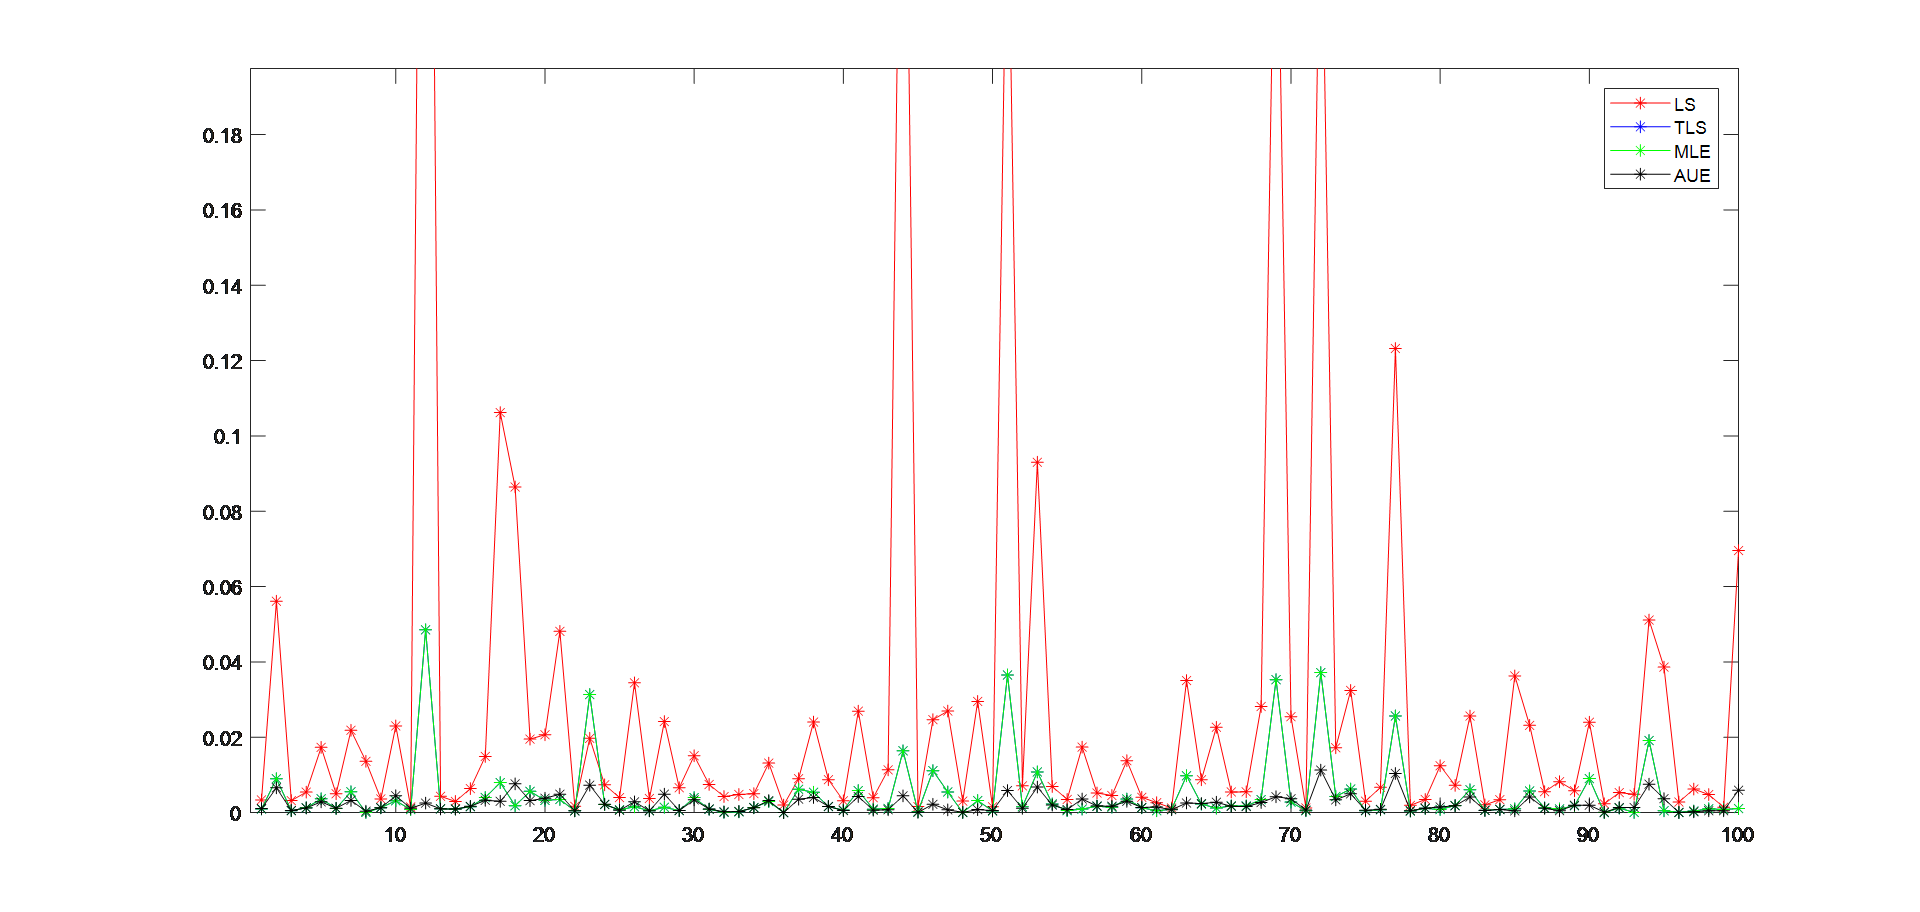
\includegraphics[width=\linewidth]{images/100MonteCarlo.png}	
} 

	\subfigure[速度相对误差图]{
	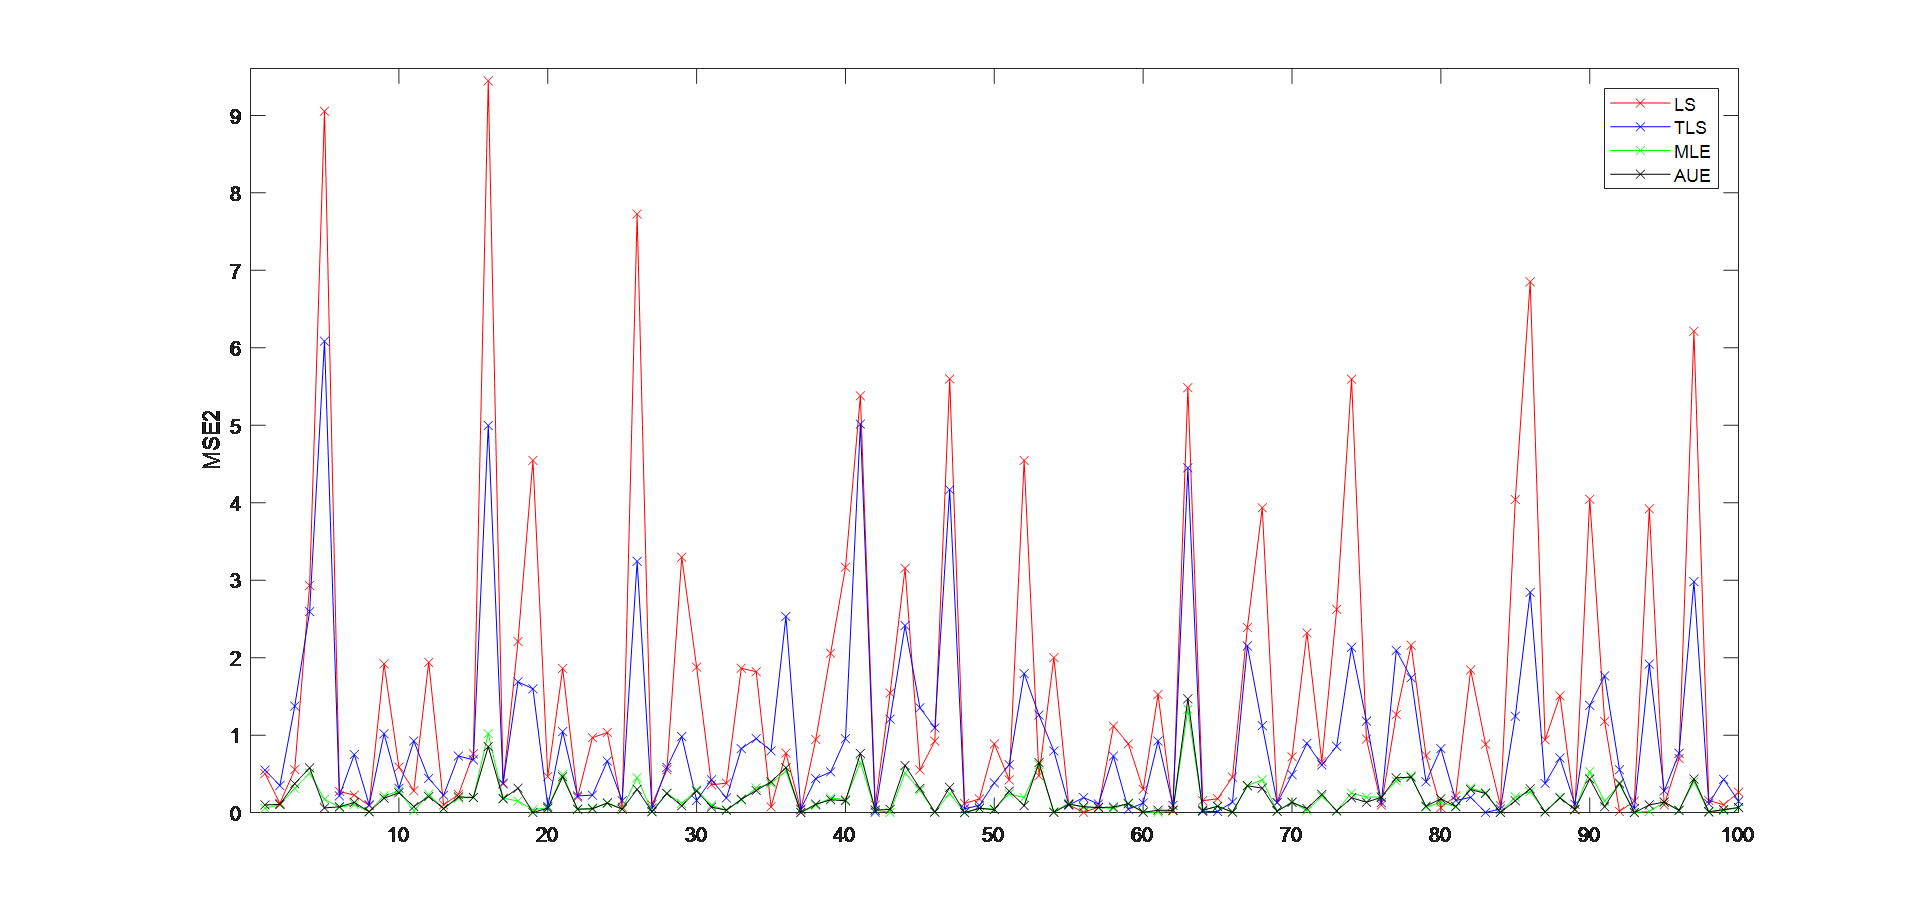
\includegraphics[width=\linewidth]{images/100MC_MSE2.png}	
}
	\caption{100次Monte Carlo实验各算法误差分析}
\end{figure}

\newpage

根据上图,在100次Monte Carlo实验中,对目标的初始状态 $\bm{X}_0$求解结果的相对误差进行比较.从距离相对误差图来看,AUE算法和MLE算法的结果相对较好,且受噪声的影响相对于其它两种算法较小,TLS算法相对于OLS算法表现的较好,但是受噪声的影响较大,不稳定.OLS算法表现结果相对较差,受噪声影响最大.从速度相对误差图来看,AUE算法和MLE算法的结果相对较好,误差范围大致在 $0 \sim 0.5$ 之间,而TLS算法和OLS算法得到的结果并不稳定,受噪声影响较大.

在不改变观测站运动状态的情况下,取 $(50km,60km,70km,0.5km/s,0.4km/s$, $ 0.2km/s)$ 做为目标的初始状态矢量,取 $\sigma=0.00005$,根据 $iT$ 时刻($T=0.1s$)前的观测数据来计算目标在 $iT$ 时刻的状态矢量 $\bm{X}_i$,得到误差图如下:
\begin{figure}[htbp]
	\centering
	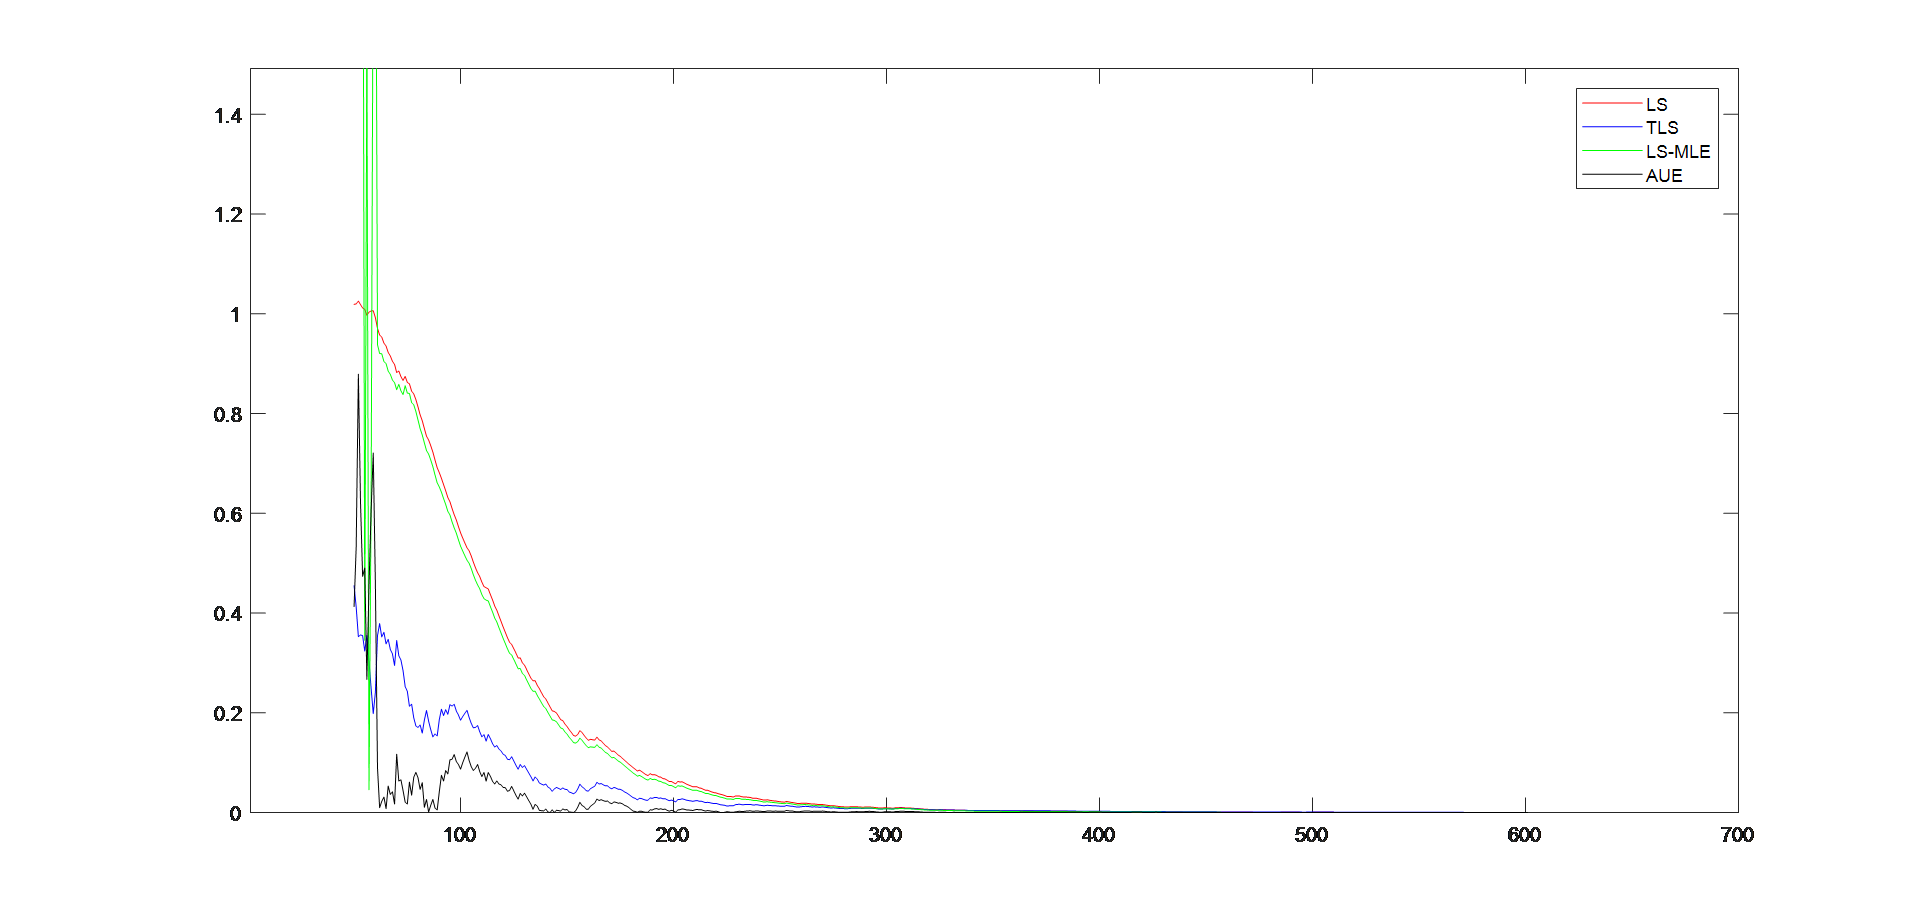
\includegraphics[width=\linewidth]{images/singleline.png}
	\caption{距离相对误差图}
\end{figure}

根据距离相对误差图分析,随着观测时间的增加各个算法求解的位置相对误差在不断减小,在15s时初步达到较为精确的定位.可以判断随着测量信息量的增多,算法对目标的运动轨迹判断变得更为准确,降低了噪声的影响,使定位更加准确.其中AUE算法和TLS算法求解的结果较好,最先得到较为准确的结果.

根据图4-3的速度相对误差图可知,随着观测时间的增加各个算法求解的速度相对误差在不断减少,但是求解得到的误差仍比较大,在15s时初步得到较为准确的结果.其中AUE算法和TLS算法最先得到较为准确的结果.
\newpage
\begin{figure}[htbp]
	\vspace{6pt}
	\centering
	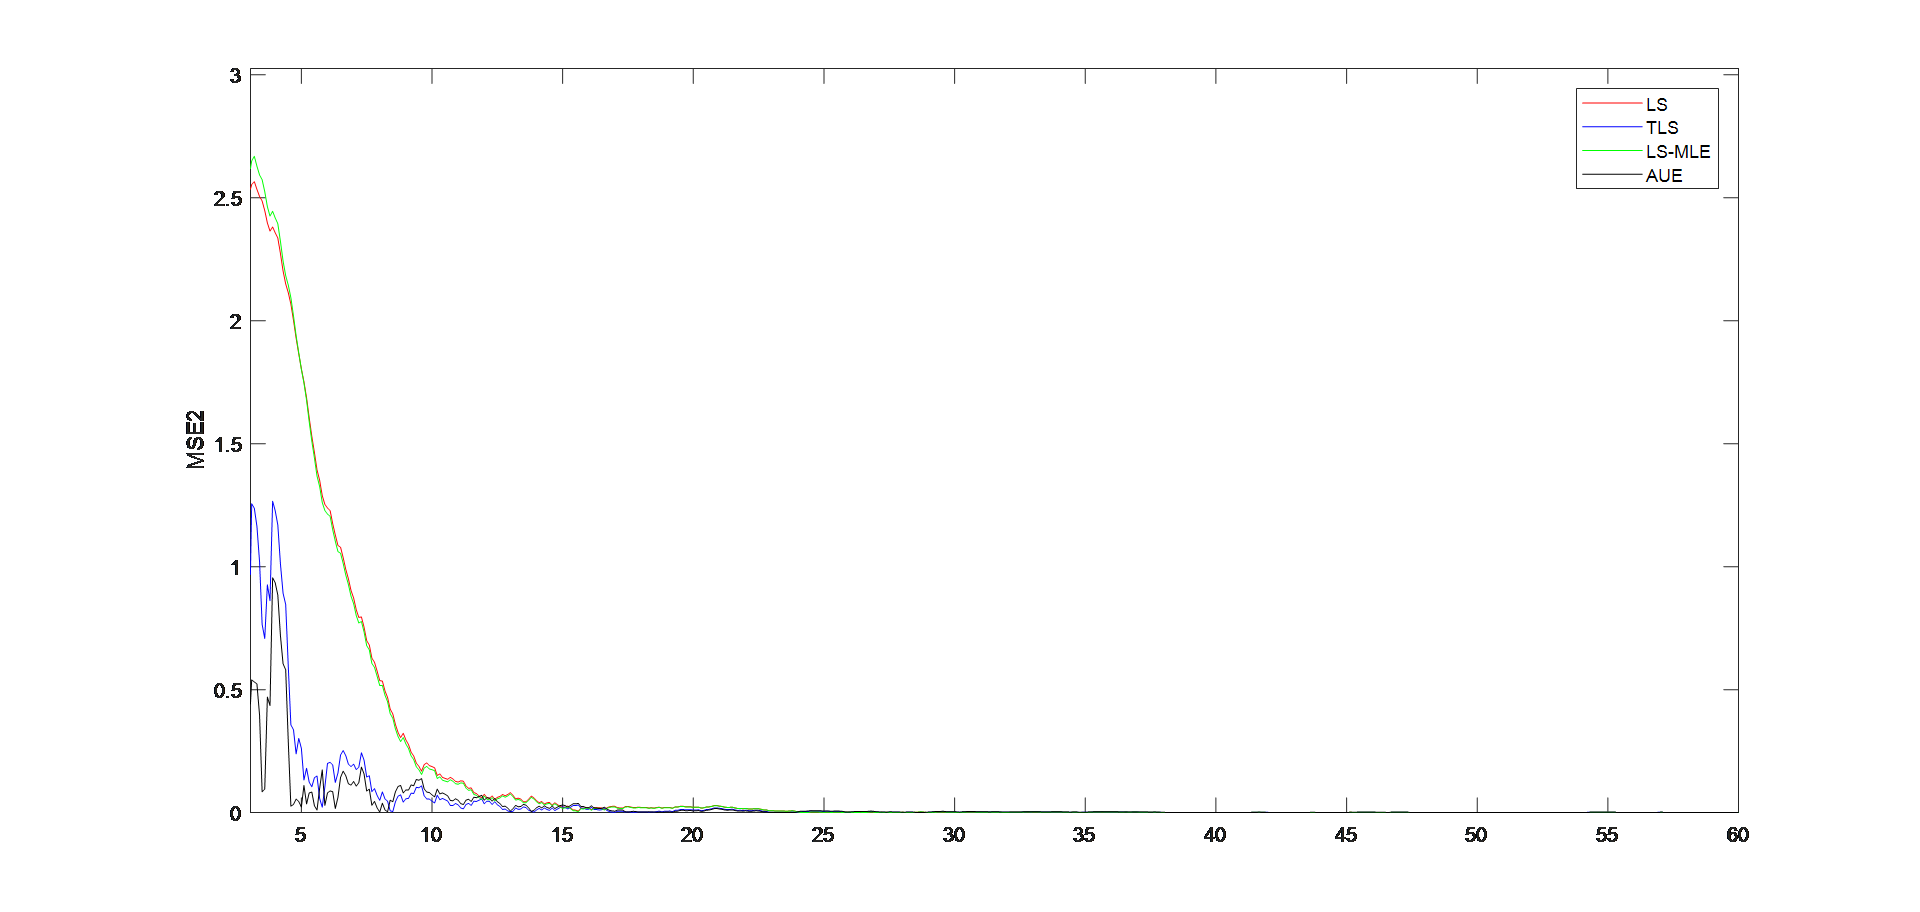
\includegraphics[width=\linewidth]{images/line_v.png}
	\caption{速度相对误差图}
\end{figure}

为了更好的分析求解情况,取出15s之后的误差结果图,判断各个定位算法的求解精度,误差结果图如图4-4和图4-5所示.

\begin{figure}[h]
	\centering
	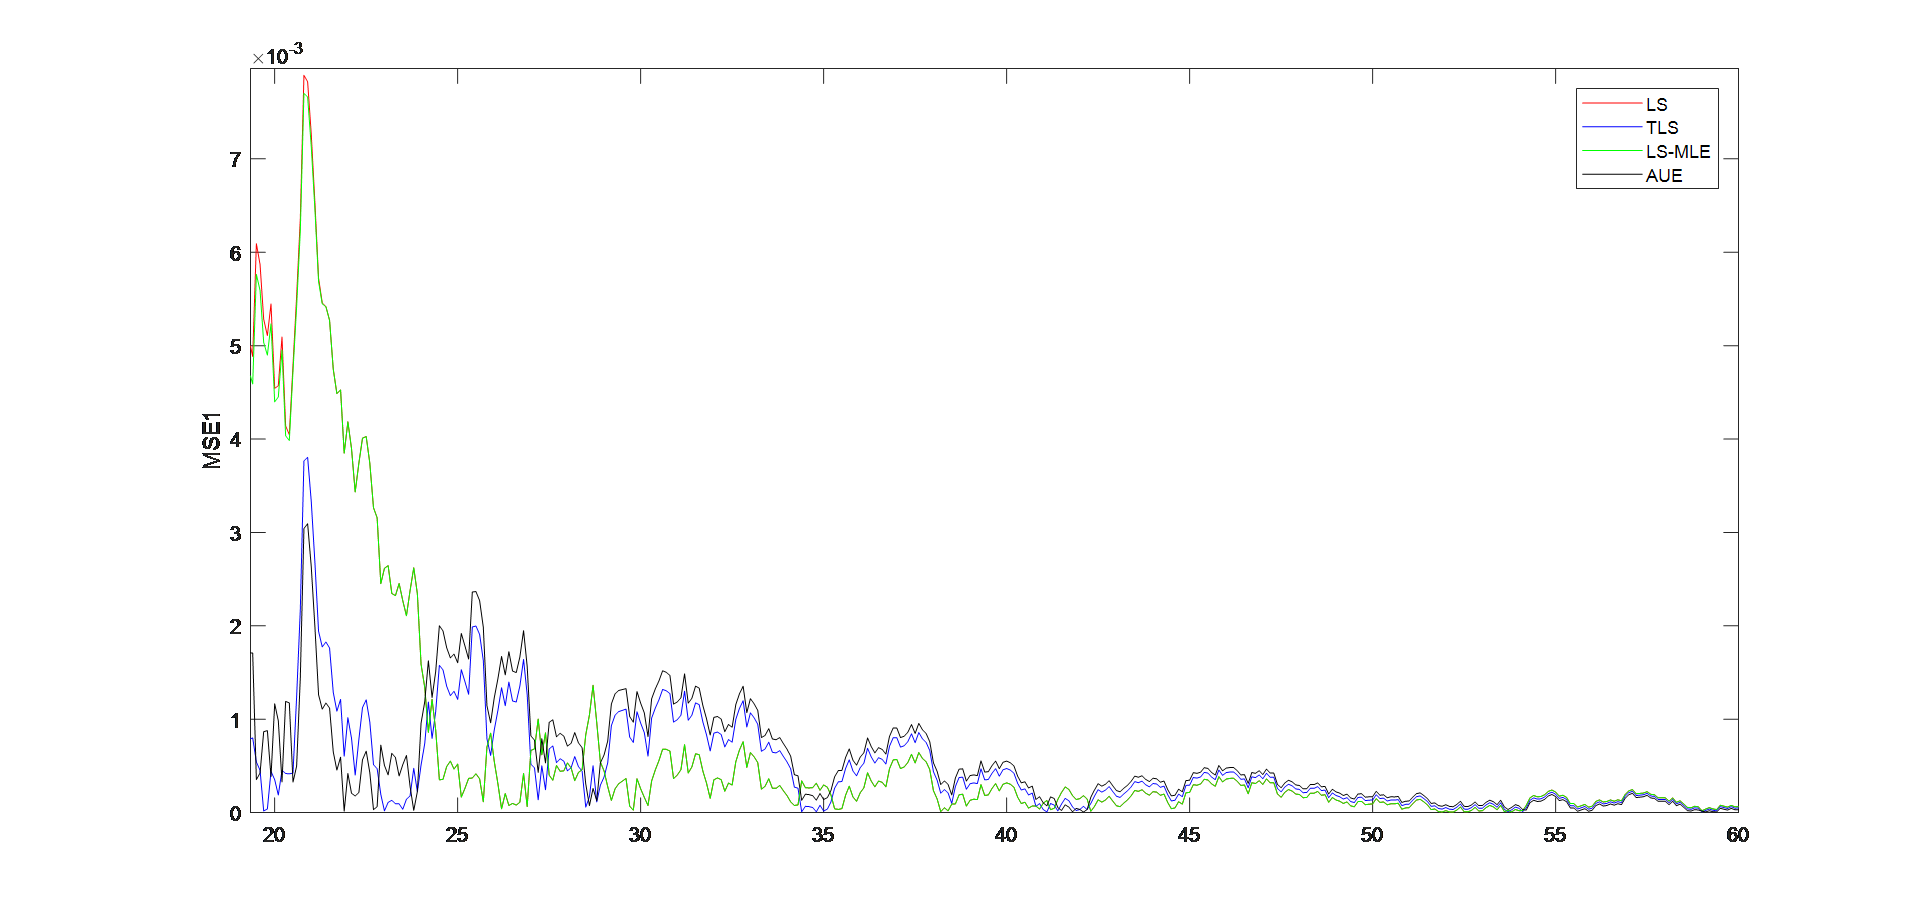
\includegraphics[width=\linewidth]{images/zoomsingleline.png}
	\caption{15s后的距离相对误差图}
\end{figure}
据图4-4和图4-5可知,在当前实验条件下,在15s之后四种算法求解得出的距离误差和速度误差都比较小,而且在40s之后,四种算法求解得到的误差没有明显区别,基本一致.
\newpage
\begin{figure}[htbp]
	\vspace{13pt}
	\centering
	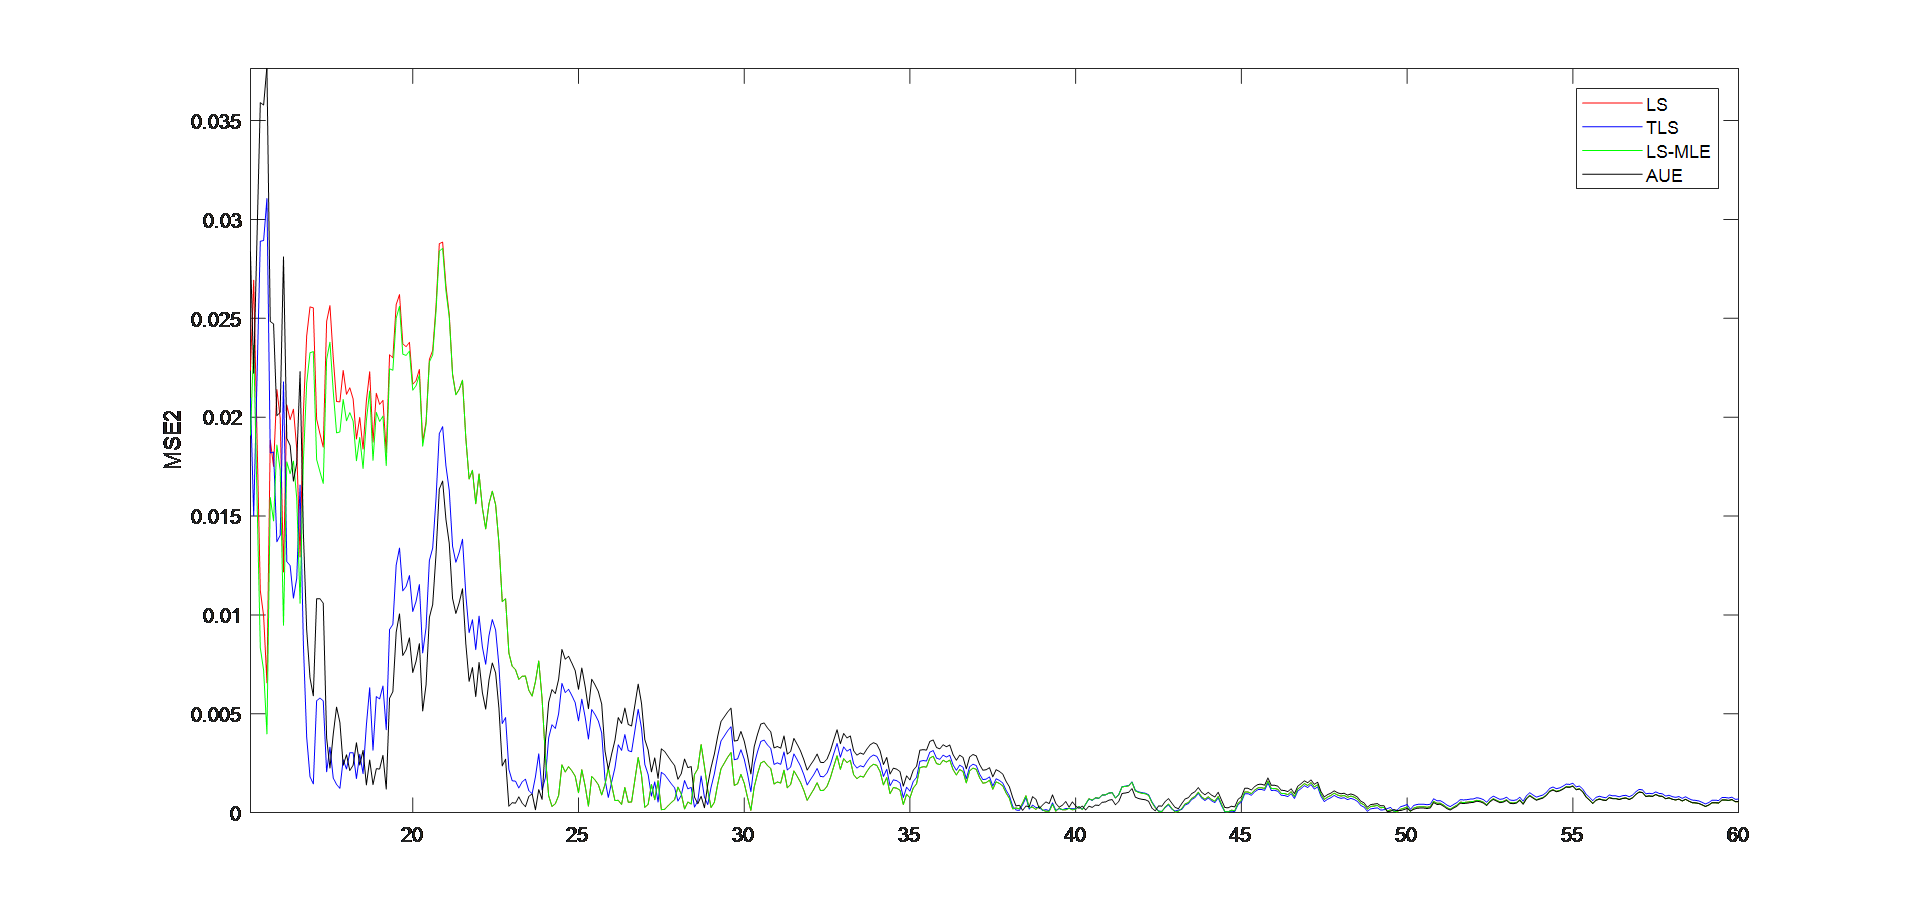
\includegraphics[width=\linewidth]{images/line_vzoom.png}
	\caption{15s后的速度相对误差图}
\end{figure}

根据以上初步实验分析可知,AUE算法对目标的轨迹求解较好,可以在相对较少测量信息的条件下得到较为精确的值.OLS算法和TLS算法对目标轨迹求解结果不稳定,容易出现较差求解结果.MLE算法在信息量足够的情况下也能得到较好的求解结果,但在信息量较少的时候求解的较差,且MLE算法的求解结果取决于初值的选取,迭代过程中产生的计算量相对较大,而且可能会出现不收敛的情况,因此在接下来的实验中暂时不考虑MLE算法.
\section{观测站与目标的距离对算法结果的影响}
为了研究观测站与目标的距离对算法的影响,考虑如下实验条件:

观测站在 $X$ 轴上运动,其加速度矢量为 $\bm{a}=(0.01,0,0)$,初始速度为 $\bm{v}_B = (0,0,0)$,目标的运动速度为 $\bm{v} = (0.3km/s,0.4km/s,0.5km/s)$.在60s的时间内,观测站从0时刻开始每隔0.1s对目标的角度信息进行一次测量,然后利用60s内观测的信息对目标的初始状态求解.在该条件下进行200次实验,其中目标的初始速度为 $\bm{v}=(0.3km/s,0.4km/s,0.5km/s)$,第一次实验时目标的初始位置坐标为 $(50km,50km,50km)$,之后每次实验目标的初始位置坐标在上一次的基础上增加 $(5km,6km,6km)$,假设每次实验测量角度的噪声相同,且取$\sigma=0.00005rad$,得到算法的求解误差图如下:
\newpage
\begin{figure}[htbp]
	\vspace{13pt}
	\centering
	\subfigure[距离相对误差图]{
	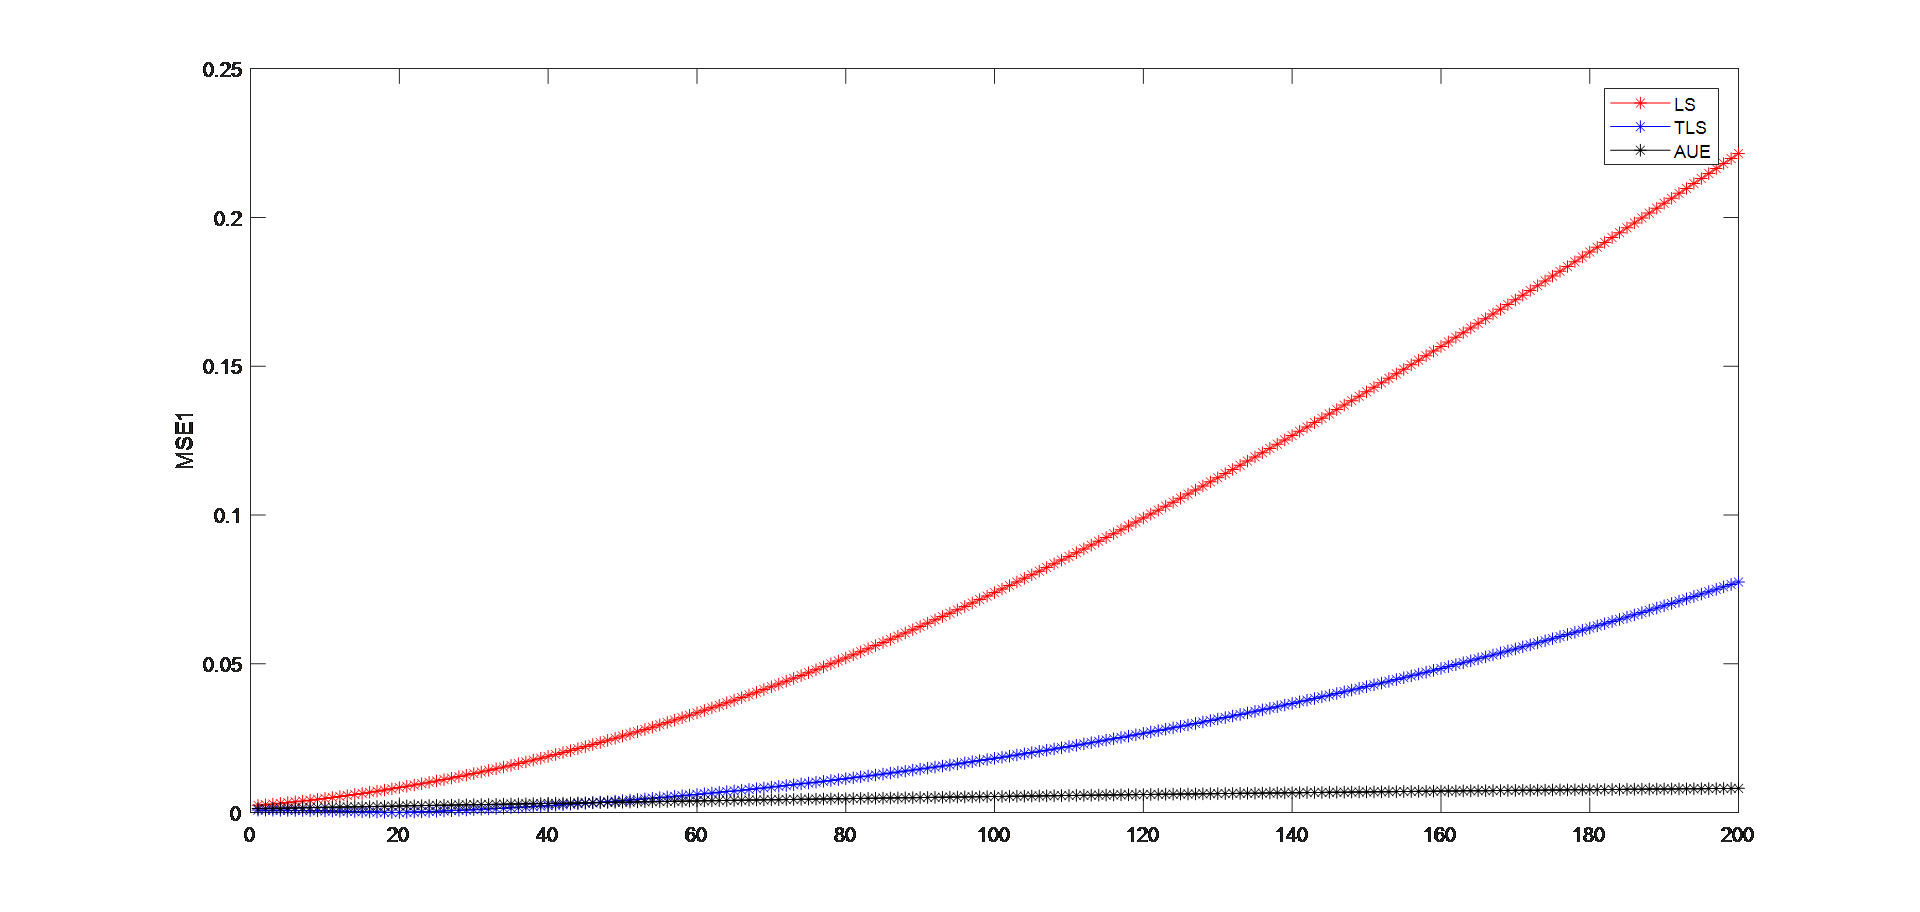
\includegraphics[width=\linewidth]{images/distence_MSE1.png}	
}

	\subfigure[速度相对误差图]{
	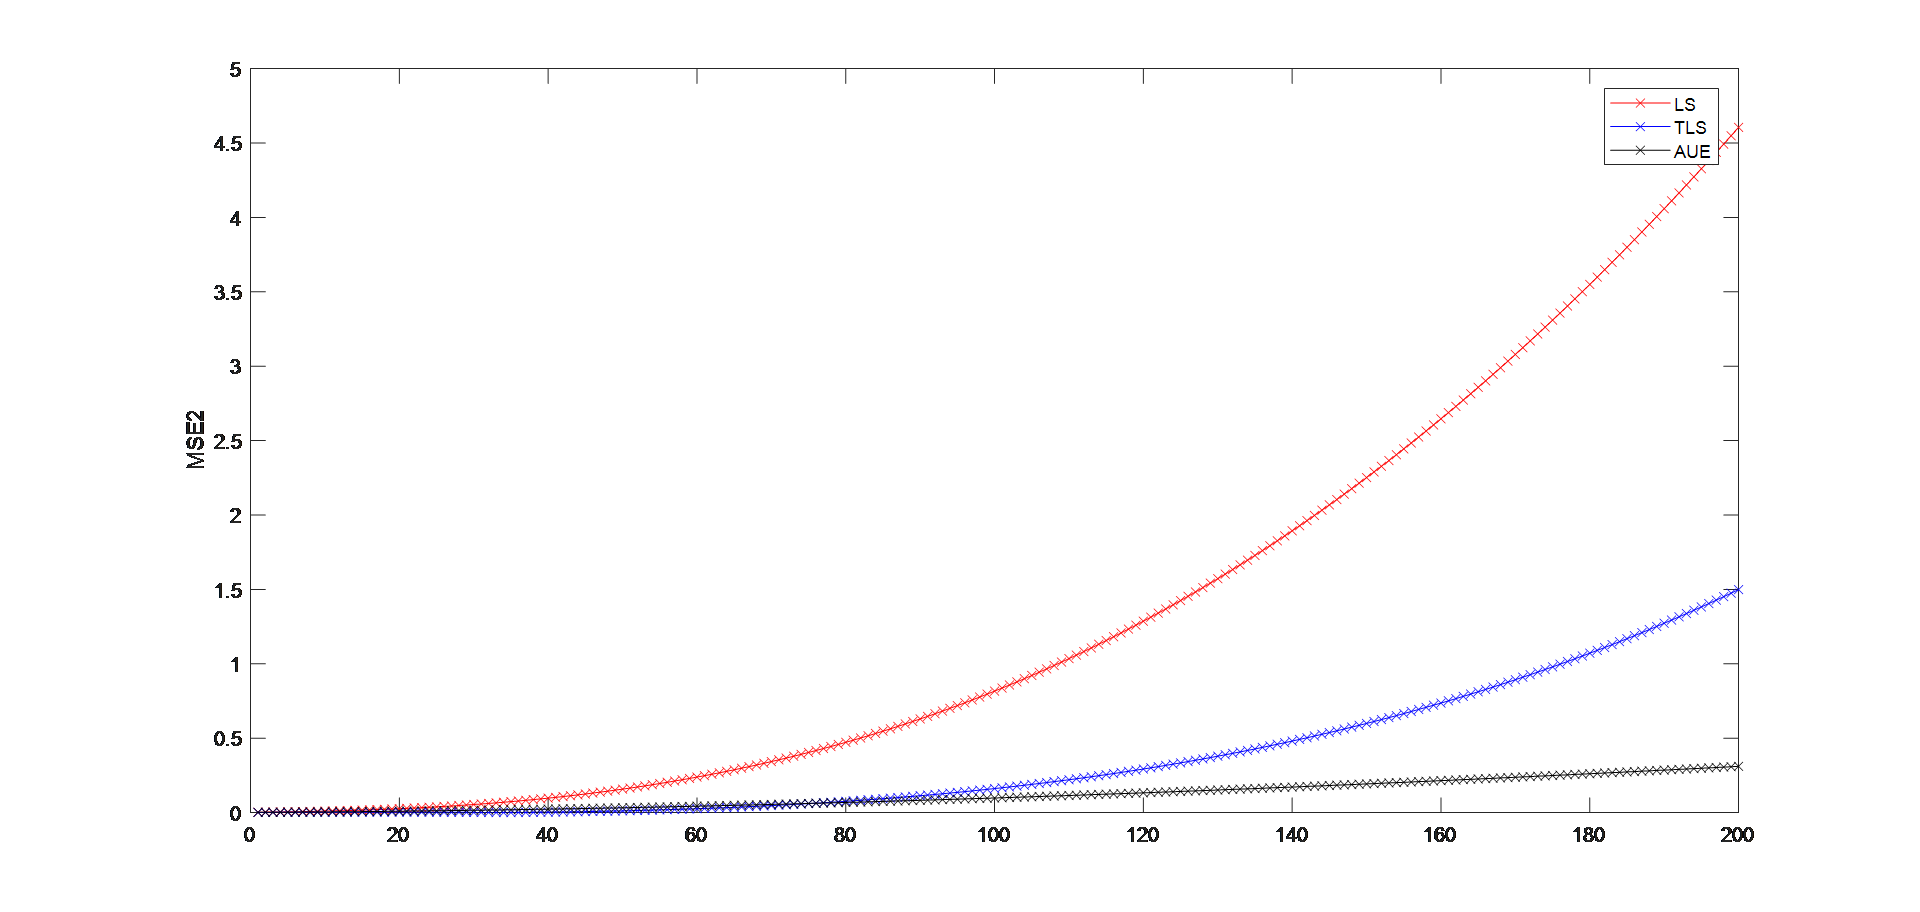
\includegraphics[width=\linewidth]{images/distence_MSE2.png}	
}
	\caption{随距离增加的误差图}
\end{figure}

从图中可以发现,在相同噪声条件下,三种算法求解得到的目标初始状态的相对误差和目标距离观测站的距离呈现一种正相关的关系.其中,OLS算法求解得到的相对误差增加最明显,TLS算法求解得到的相对误差大概在目标初始位置距离观测站约500km时才开始缓慢增加,AUE算法求解得到的相对误差随距离的增加相对于OLS算法和TLS算法增加的并不明显.出现该结果的原因可能是,在目标和观测站距离较近时,观测站每0.1s测得的角度信息的差值较大,受噪声的影响相对较小,因此计算得到的相对误差较小.但是当目标和观测站之间的距离不断变大时,观测站测得的方位角及仰角的数据较为紧凑,差值较小,受噪声的影响较大,因此计算得到的相对误差变大.不过AUE算法做为一种无偏估计算法,受噪声影响程度比其它两种算法小.

三种算法对距离的求解估计精度较高,对速度的估计精度较低,这可能是由于观测角度存在噪声的影响使得测得的目标的运动方向在不断改变,从而使得算法对目标速度的估计存在较大的偏差.

\begin{figure}[htbp]
	\centering
	\subfigure[距离相对误差]{
	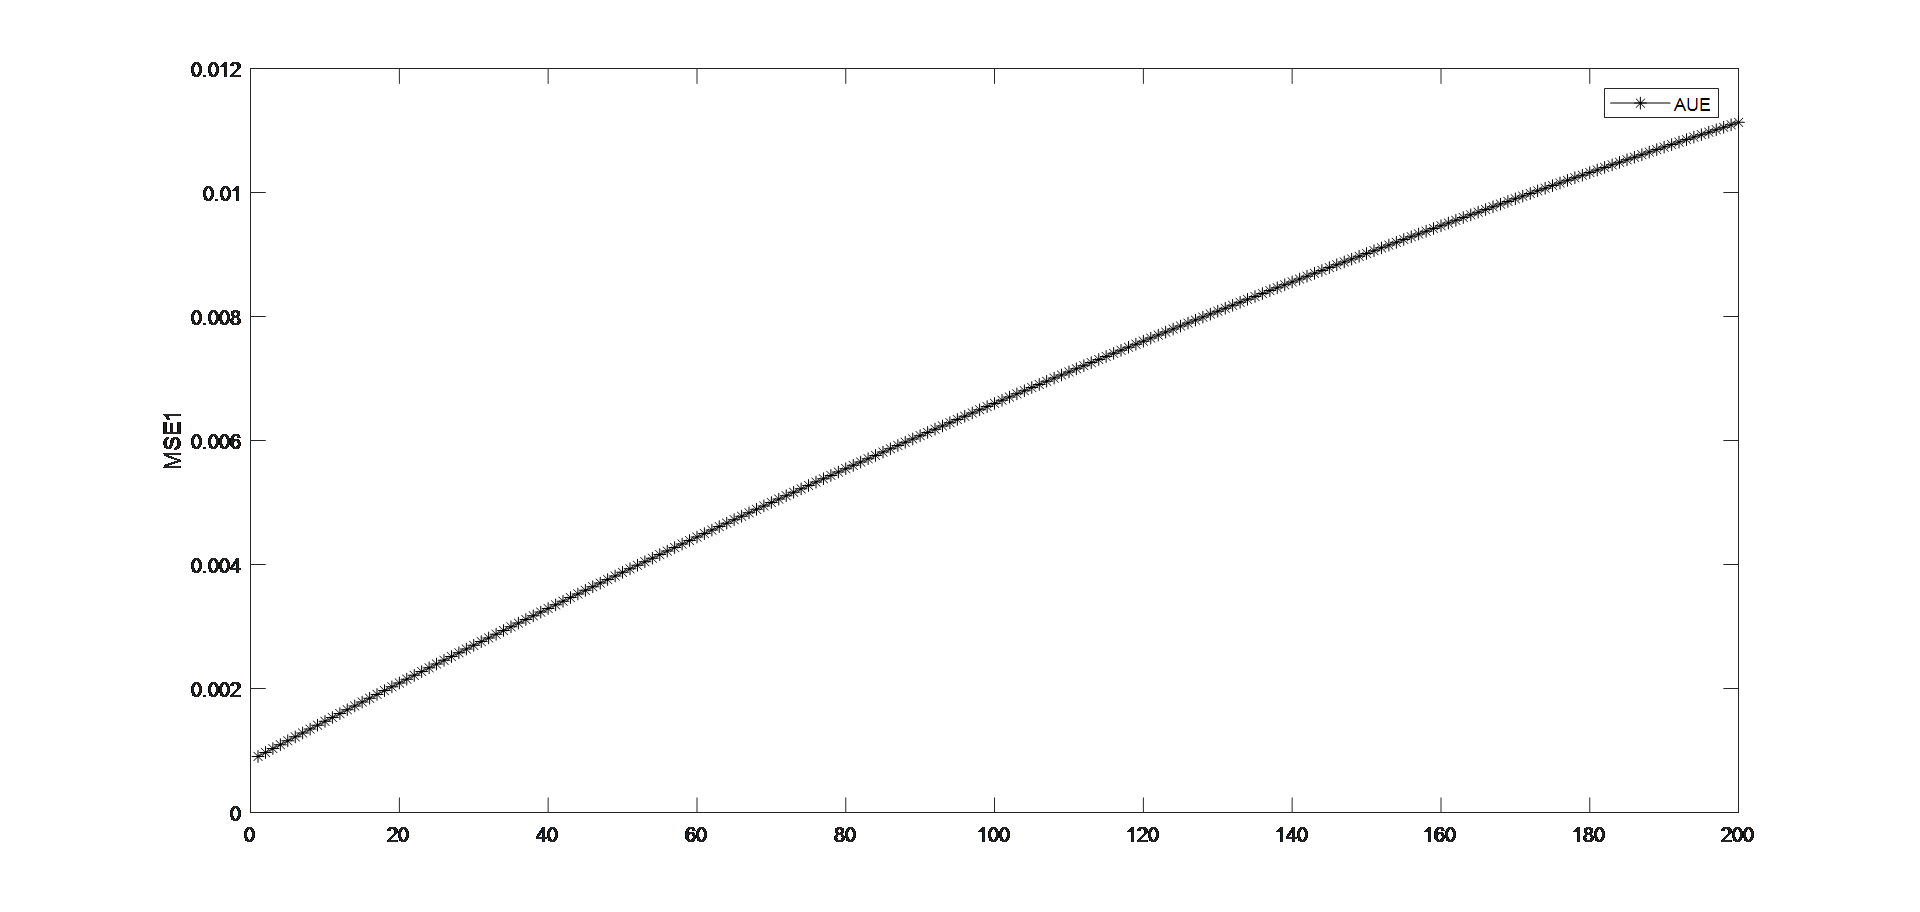
\includegraphics[width=\linewidth]{images/AUE_MSE1.png}
}
	
	\subfigure[速度相对误差]{
	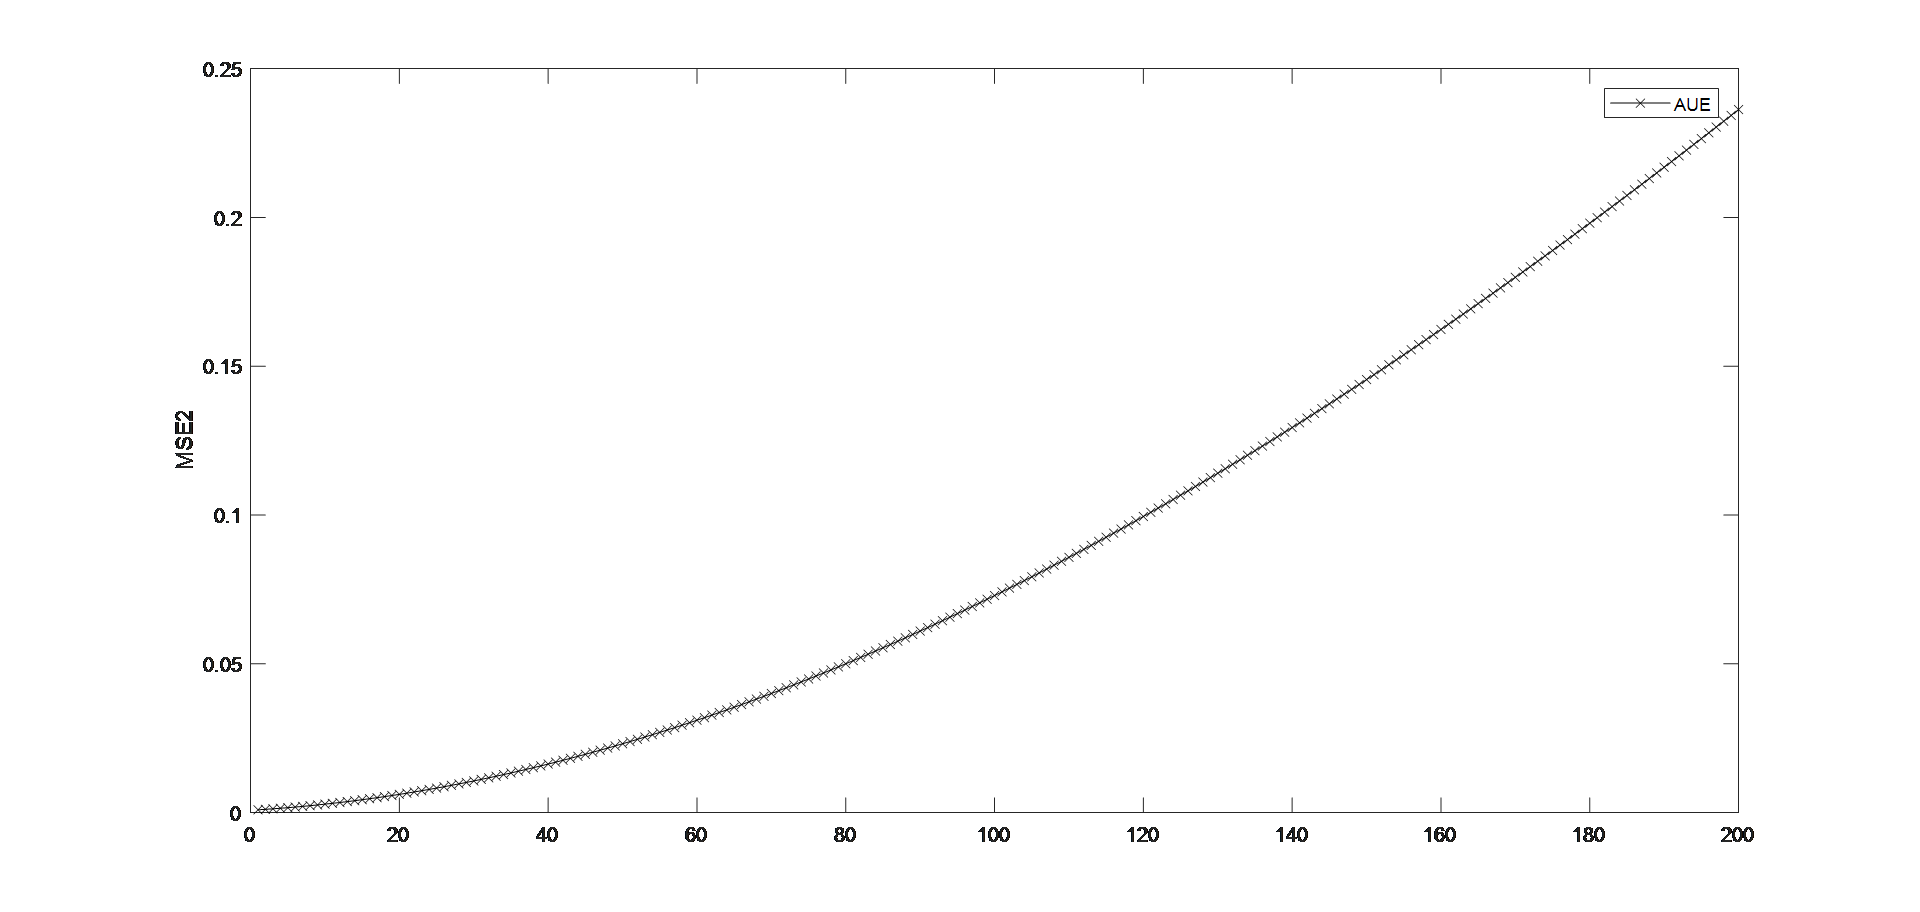
\includegraphics[width=\linewidth]{images/AUE_MSE2.png}	
}
	\caption{AUE算法随距离增加的计算误差图}
\end{figure}
图4-7将AUE算法随目标到观测站距离增加求解结果误差图单独画出,可以看到随距离增加算法的相对误差也在增加,且速度误差相对较大.
\section{方位角及仰角对算法结果的影响}
保持观测站运动状态不变,给定目标的初始位置为 $(500km,600km,400km)$,在第一次仿真实验中目标的速度为 $\bm{v}=(0.3km/s,0.2km/s,0.1km/s)$,取 $\sigma=0.00005rad$,每次使目标的初始速度增加 $(0,0,0.1km/s)$,在相同噪声条件下共进行20组仿真实验,得到求解结果的误差图:
\begin{figure}[htbp]
	\centering
	\subfigure[距离相对误差图]{
	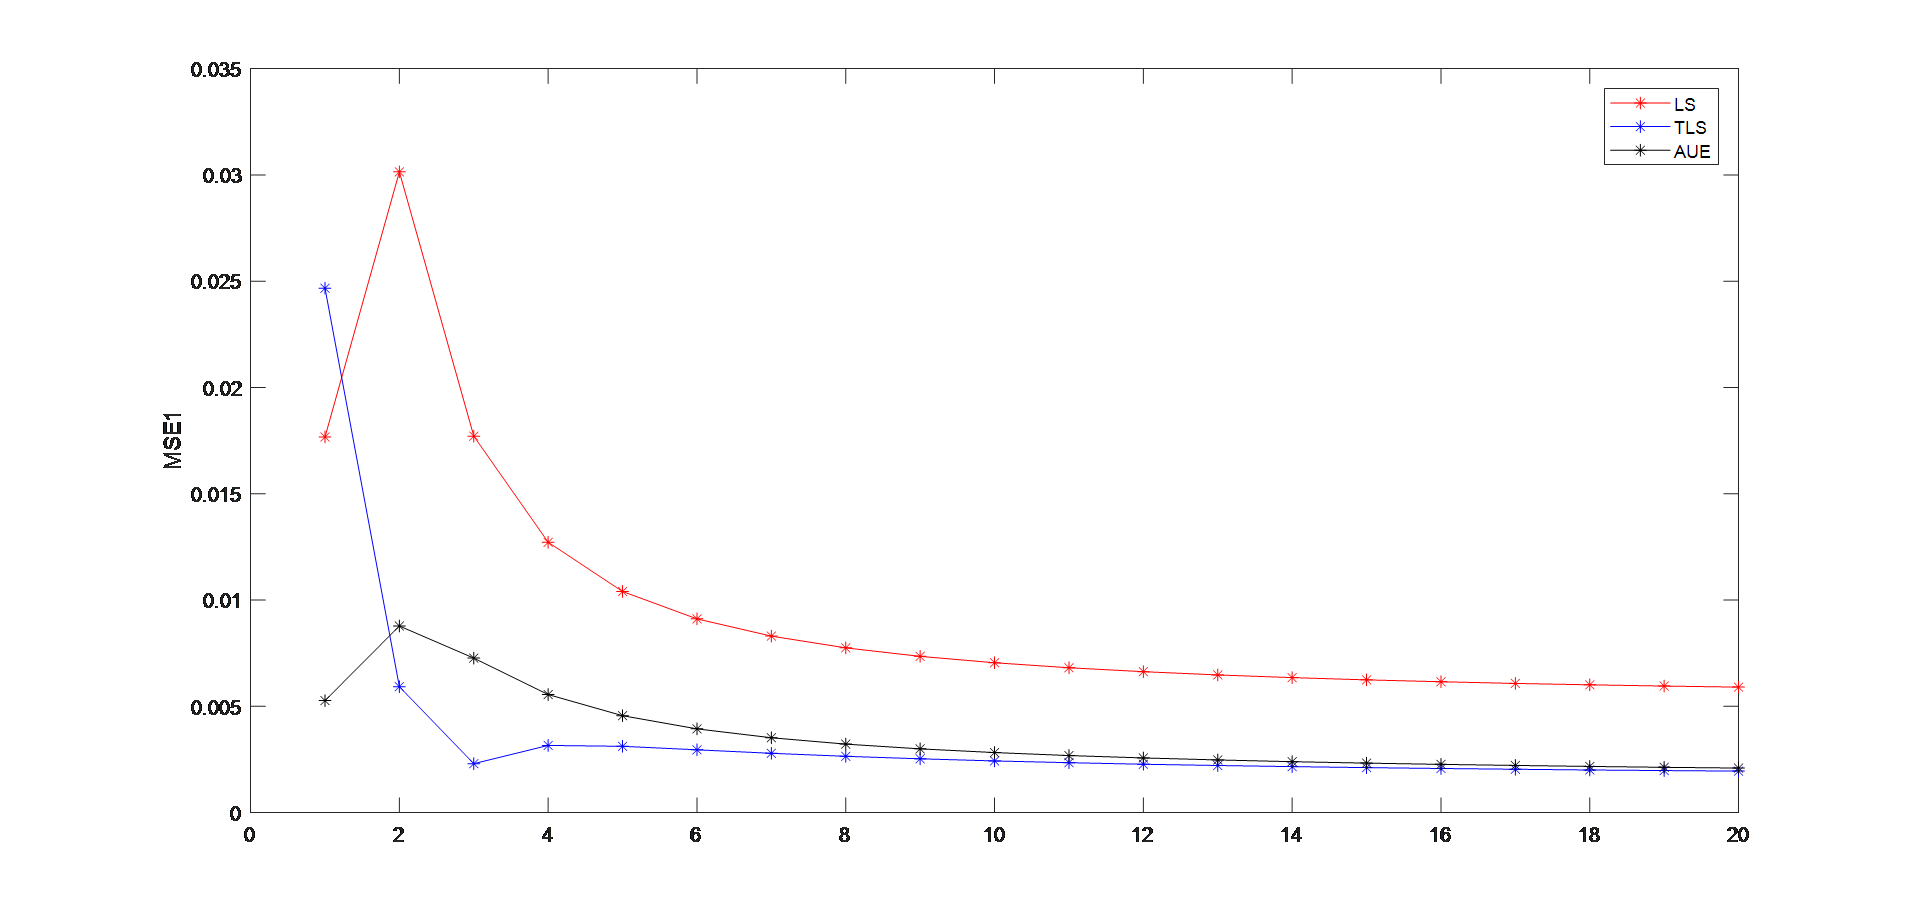
\includegraphics[width=0.93\linewidth]{images/elevation_MSE1.png}	
}

	\subfigure[速度相对误差图]{
	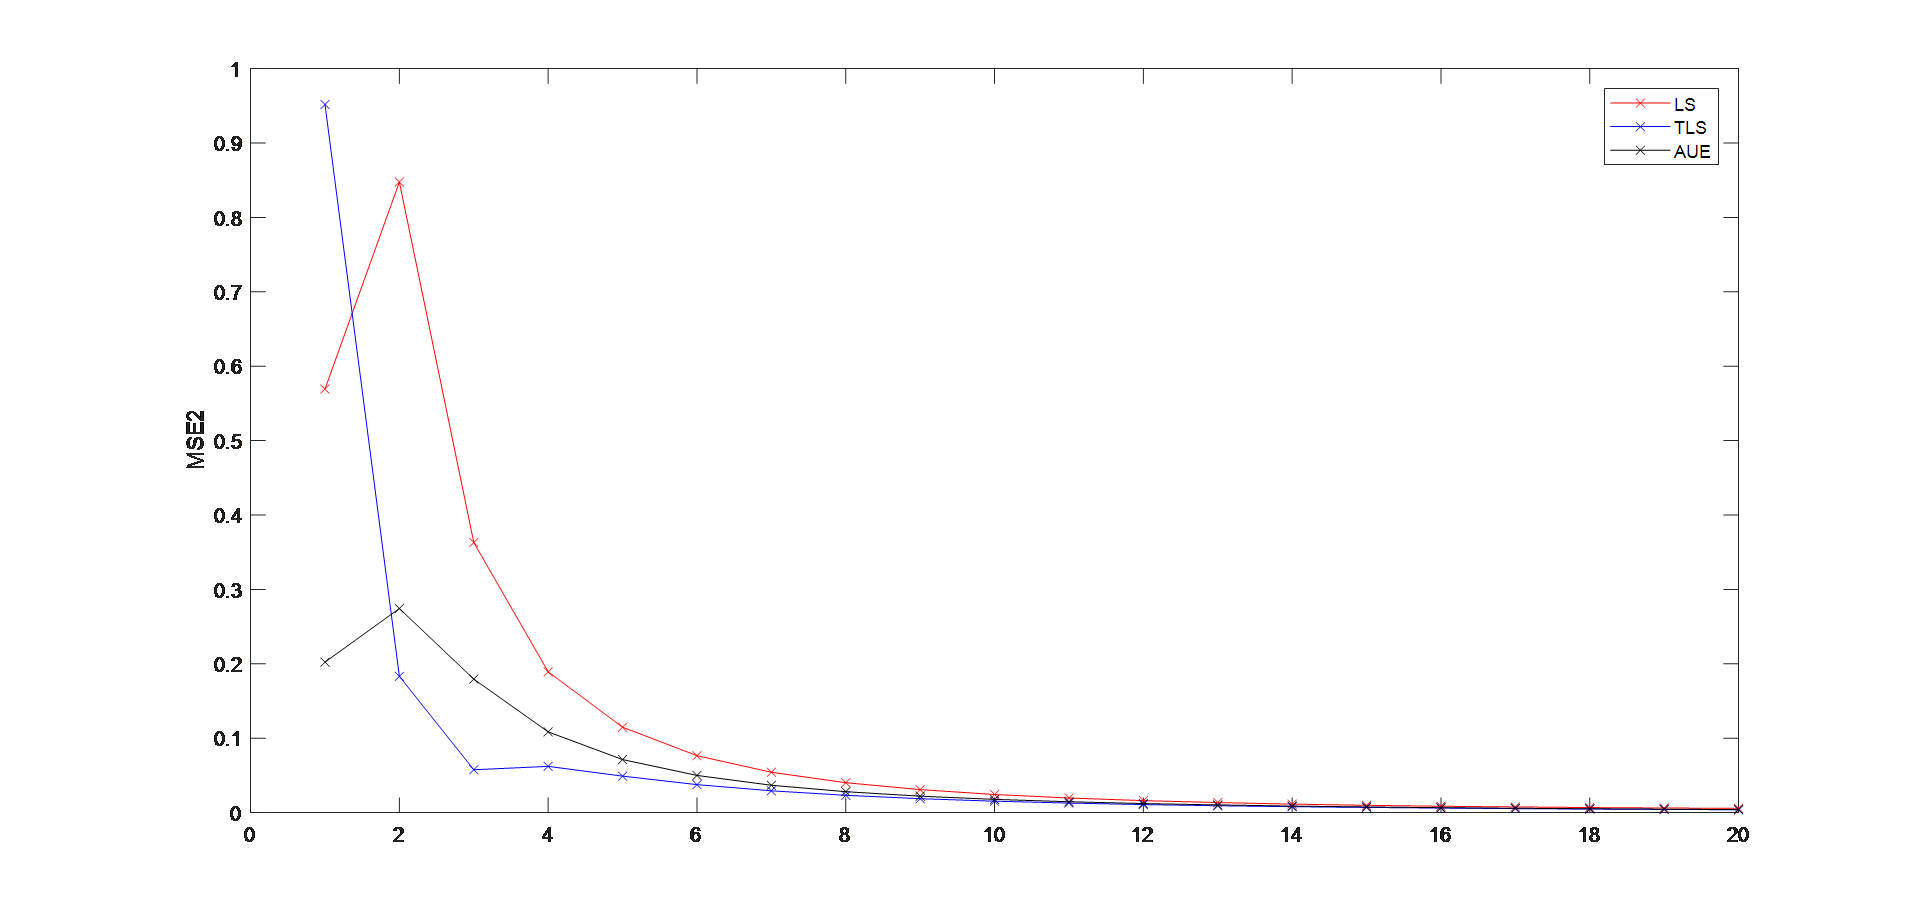
\includegraphics[width=0.93\linewidth]{images/elevation_MSE2.png}	
}
	\caption{仰角变化对结果的影响}
\end{figure}

在上述仿真实验条件中,改变第一次实验中目标的速度为 $\bm{v} = (0.1km/s,0.2km/s,0)$,速度每次增加 $(0.1km/s,0.2km/s,0)$,进行20组仿真实验,得到求解结果的误差图:
\begin{figure}[htbp]
	\centering
	\subfigure[距离相对误差图]{
	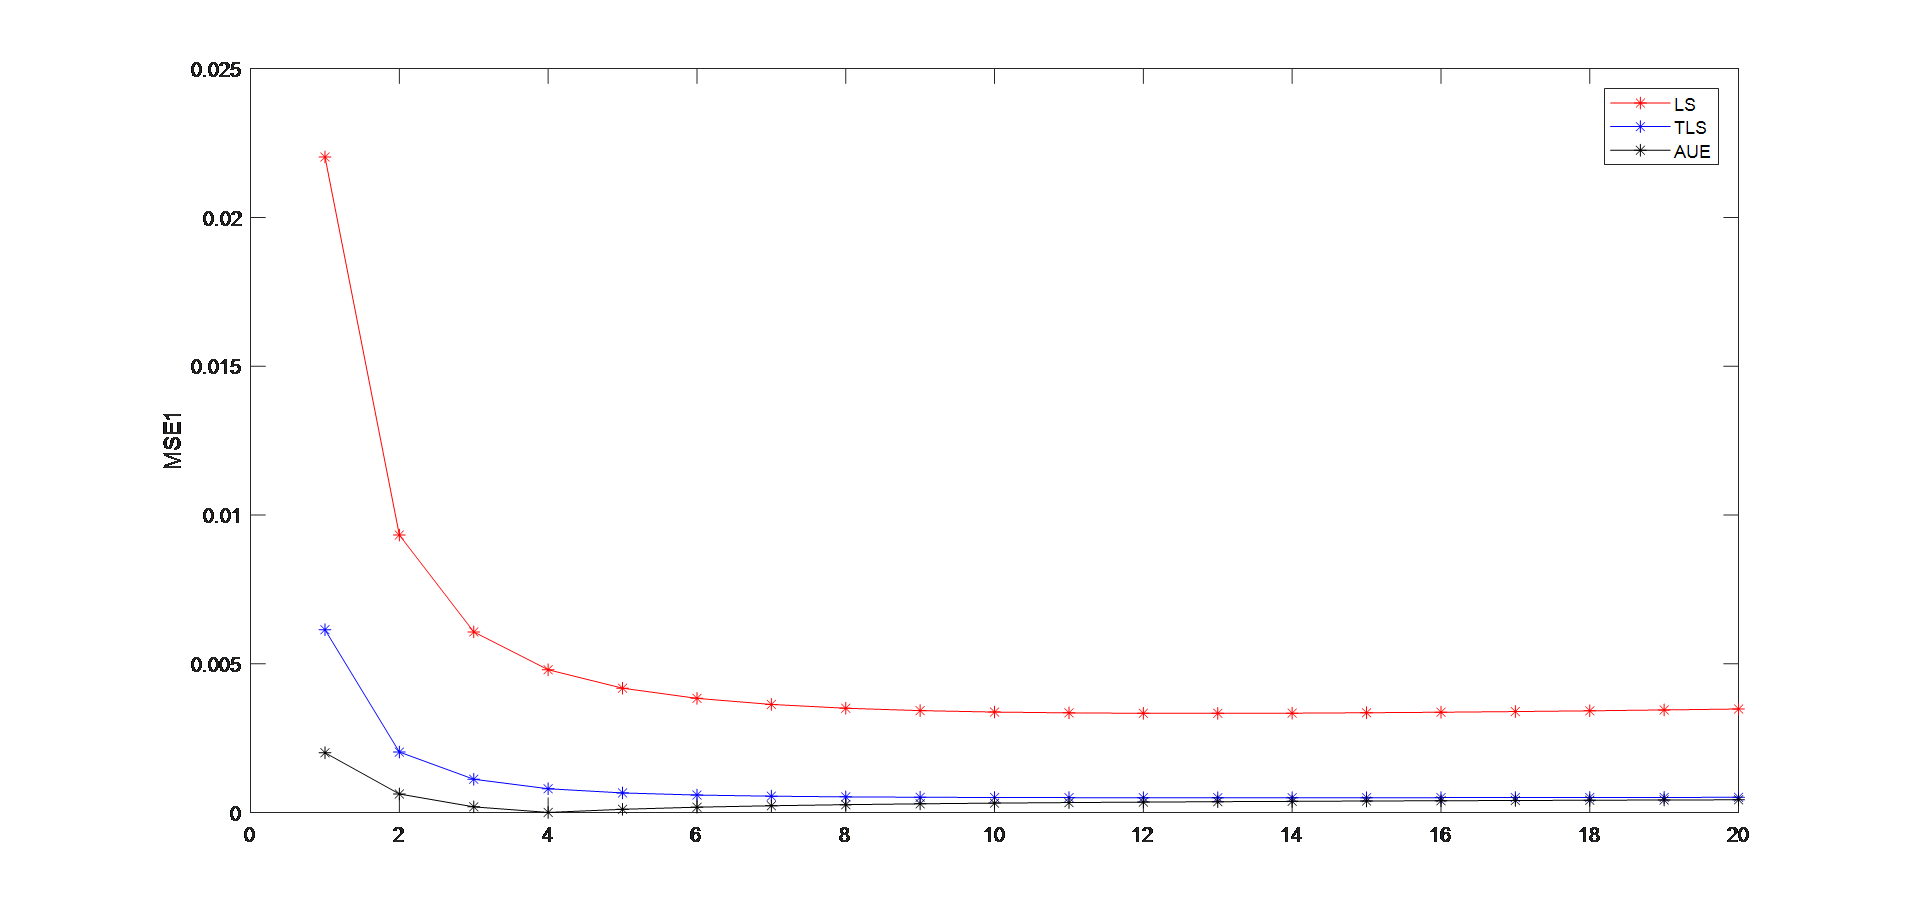
\includegraphics[width=\linewidth]{images/azimuth_MSE1.png}	
}

	\subfigure[速度相对误差图]{
	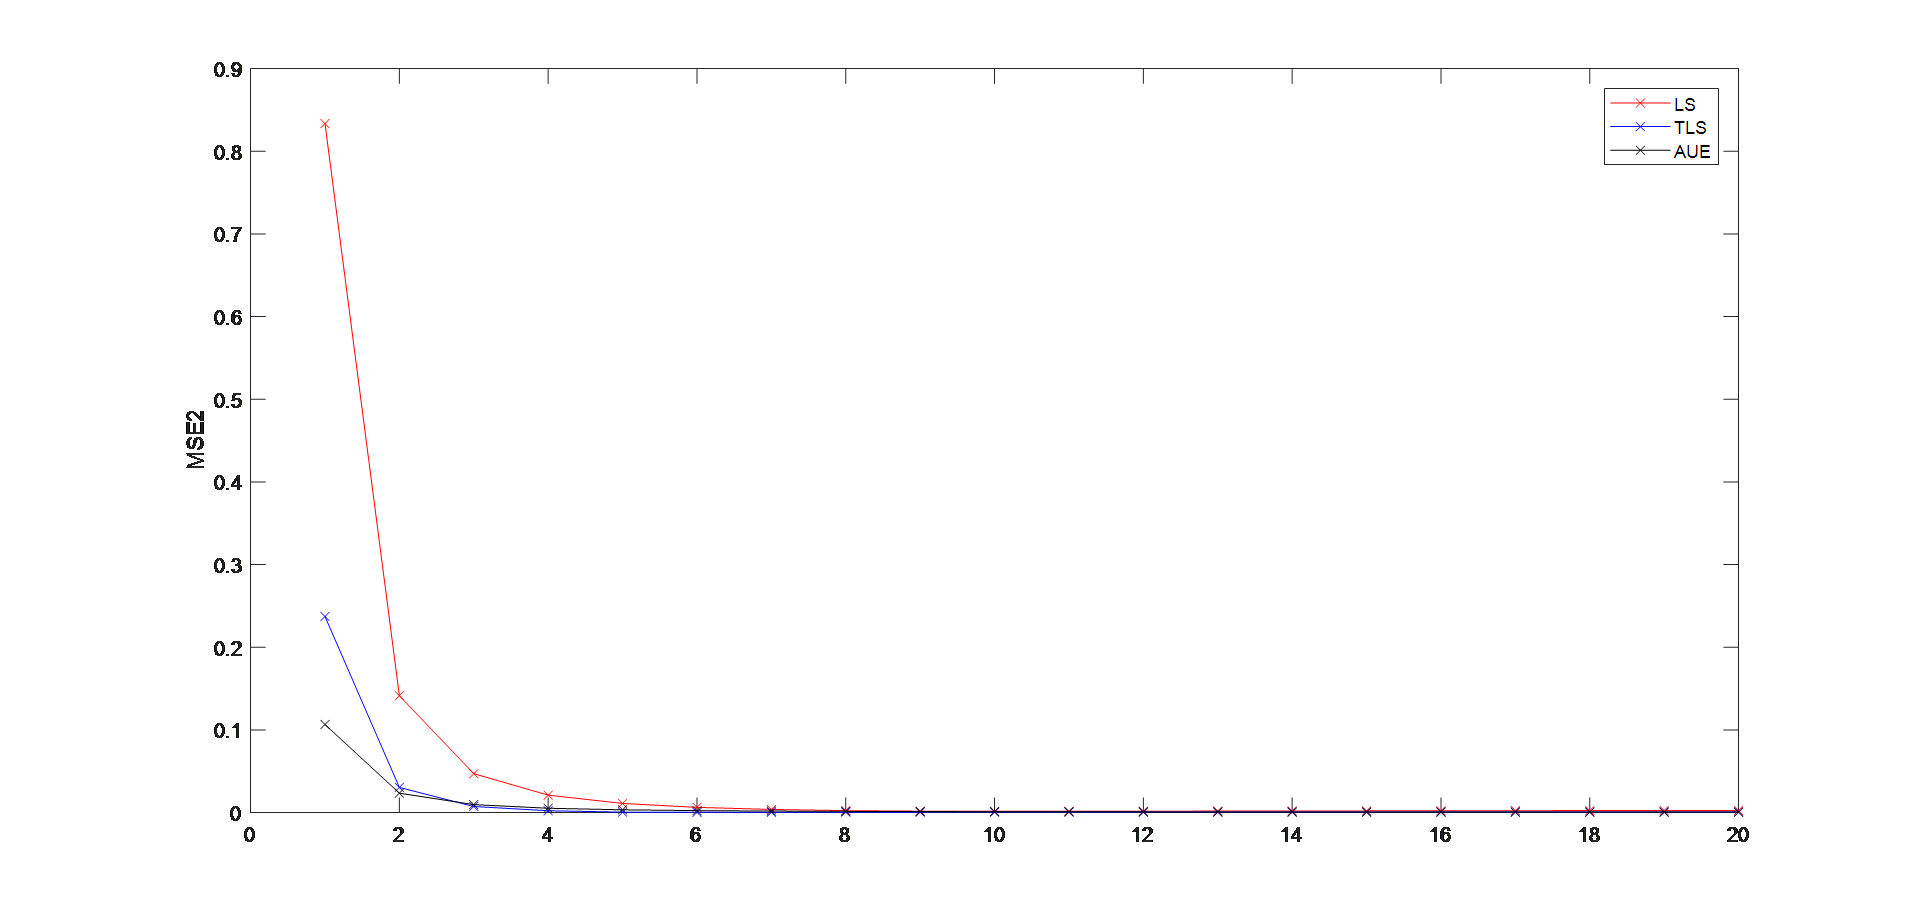
\includegraphics[width=\linewidth]{images/azimuth_MSE2.png}	
}
	\caption{方位角变化对结果的影响}
\end{figure}

从结果可以看出,当仰角间差值增大,即测量的相邻两次的仰角数据的差值变大,求解结果便会更加精确.同样的当方位角间差值增大,求解结果也会更加精确.这是因为当差值变大时,噪声对测量的结果影响变小,从而求解结果变得更加准确.
\section{测量误差对算法结果的影响}
保持观测站的运动状态不变,给定目标的速度为 $\bm{v} = (0.3km/s,0.4km/s,0.5km/s)$,在 $(x_0,y_0,z_0) \in [0,300km]\times[0,300km]\times[0,300km]$ 范围内随机选择做为初始位置,进行100次Monte Carlo实验,并分别取$\sigma=0.0005rad,\sigma=0.0001rad,\sigma=0.00005rad$,做出算法误差图.
\begin{figure}[htbp]
	\centering
	\subfigure[距离相对误差图]{
	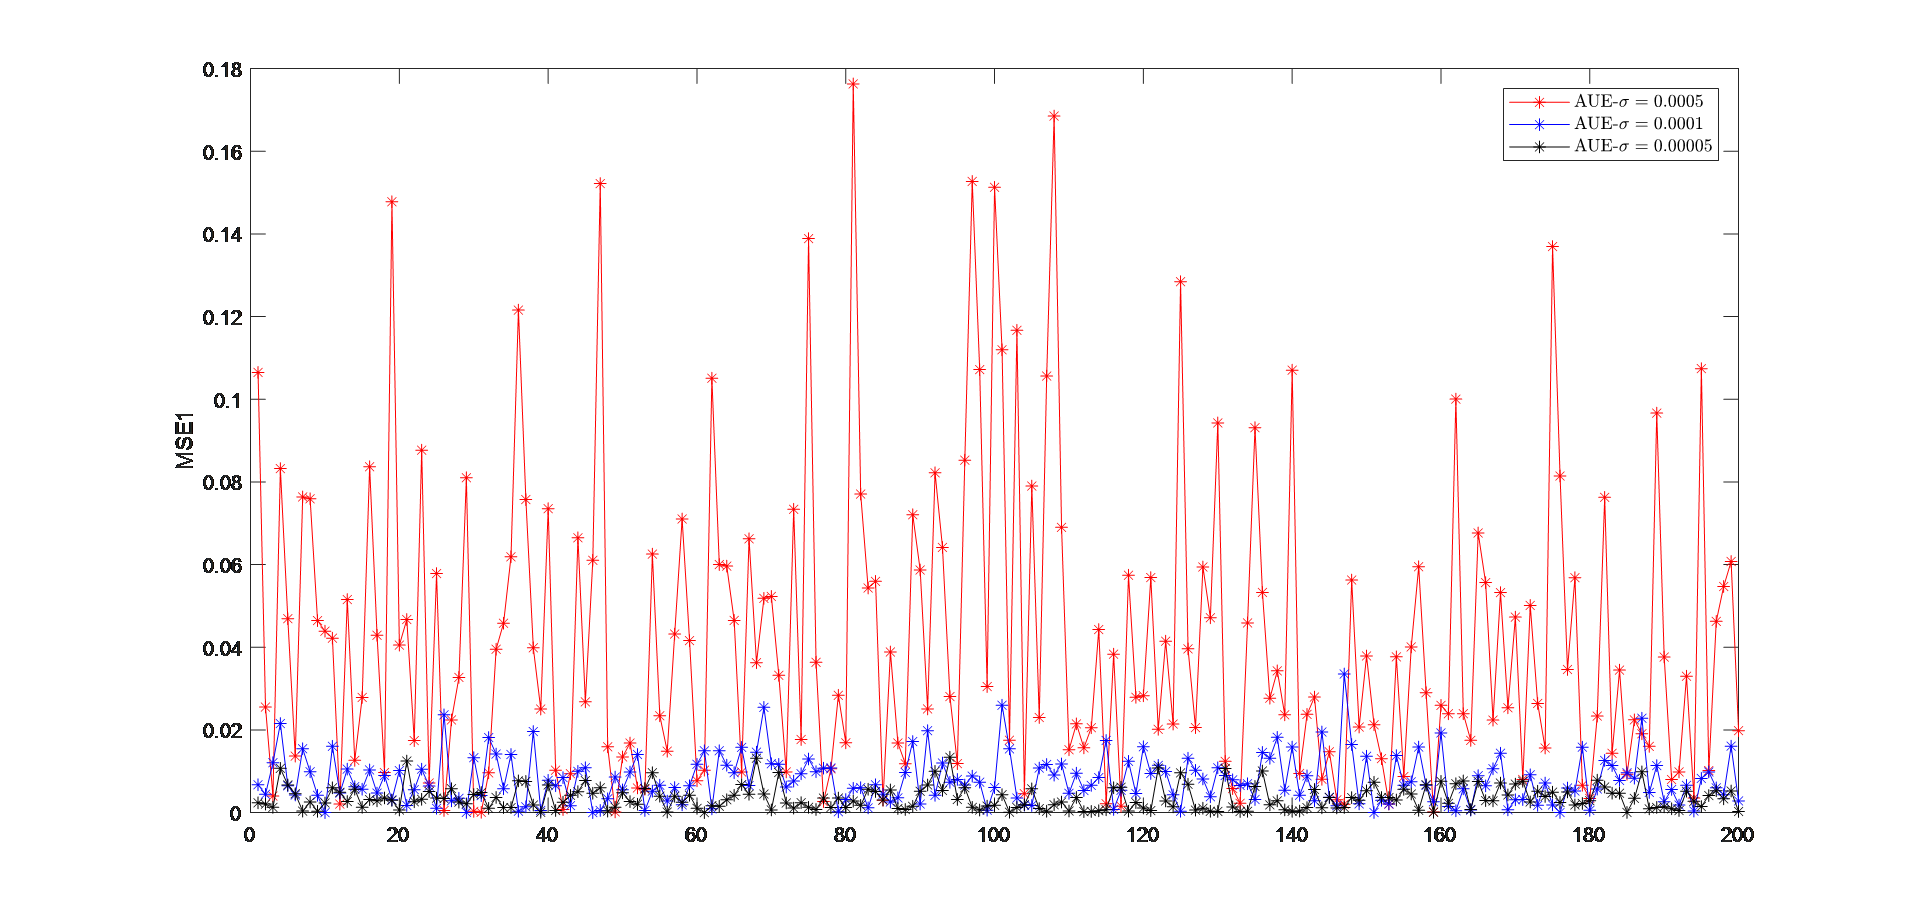
\includegraphics[width=0.93\linewidth]{images/sigma_MSE1.png}
}

	\subfigure[速度相对误差]{
	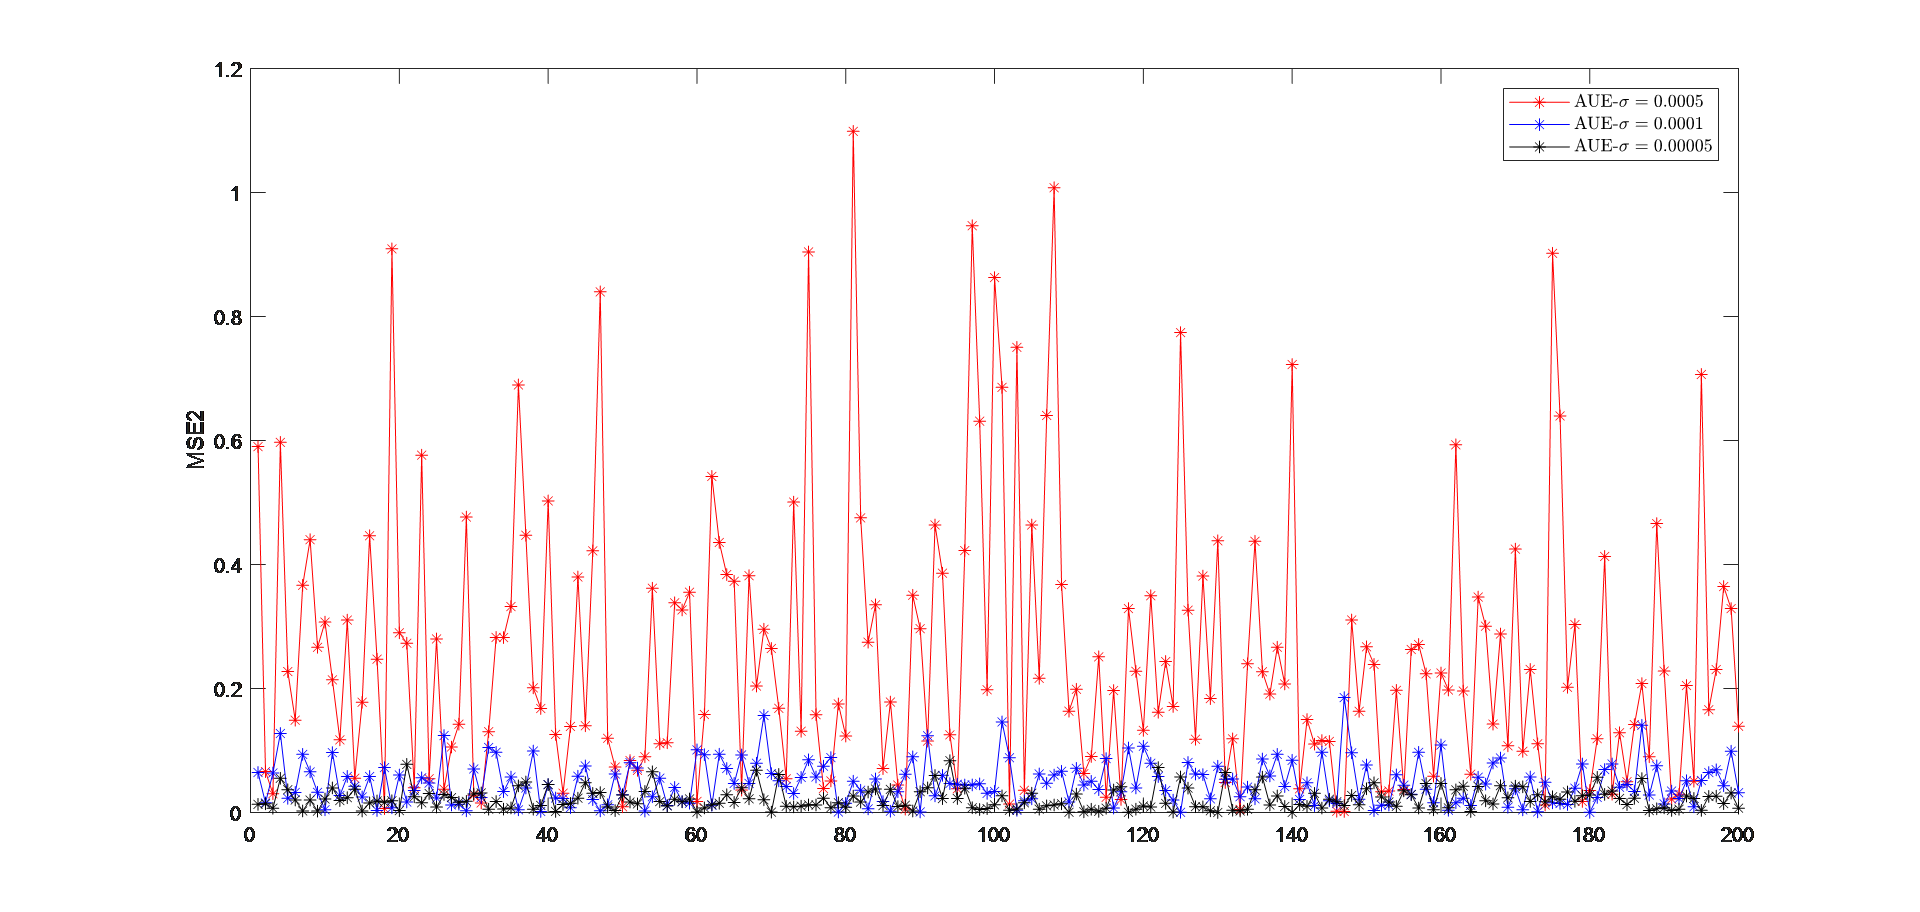
\includegraphics[width=0.93\linewidth]{images/sigma_MSE2.png}	
}
	\caption{AUE算法在不同测量误差下求解误差}
\end{figure}

由于TLS算法和AUE算法易受噪声影响,故只研究噪声对AUE算法的影响.根据上图结果可以看出,在随着测量误差的增大,AUE算法的求解结果相对误差变化幅度较大.距离相对误差的变化相对于速度相对误差的变化较小,但仍有较大误差.出现该情况的原因可能是由于目标与观测站的距离相对较大,使得真实的方位角及仰角变化不大,即实际的方位角的极差较小,仰角间的极差也相对较小,所以当噪声误差相对较大时便会对测量值产生较大的影响,使得计算得到的误差相对较大.
% 结论:在结论相应的 TeX 文件处进行结论部分的撰写
%%
% The BIThesis Template for Bachelor Graduation Thesis
%
% 北京理工大学毕业设计(论文)结论 —— 使用 XeLaTeX 编译
%
% Copyright 2020 Spencer Woo
%
% This work may be distributed and/or modified under the
% conditions of the LaTeX Project Public License, either version 1.3
% of this license or (at your option) any later version.
% The latest version of this license is in
%   http://www.latex-project.org/lppl.txt
% and version 1.3 or later is part of all distributions of LaTeX
% version 2005/12/01 or later.
%
% This work has the LPPL maintenance status `maintained'.
%
% The Current Maintainer of this work is Spencer Woo.
%
% Compile with: xelatex -> biber -> xelatex -> xelatex

\addcontentsline{toc}{chapter}{结~~~~论}
\chapter*{\vskip 10bp\textmd{结~~~~论} \vskip -6bp}

% 在结论部分的子标题不需要序号,加上 * 即可(一个例子如下)
% \section*{结论段落标题}

% 这里插入一个参考文献,仅作参考


% 参考文献:如无特殊需要,参考文献相应的 TeX 文件无需改动,添加参考文献请使用 BibTeX 的格式
%   添加至 misc/ref.bib 中,并在正文的相应位置使用 \cite{xxx} 的格式引用参考文献
%%
% The BIThesis Template for Bachelor Graduation Thesis
%
% 北京理工大学毕业设计(论文)参考文献 —— 使用 XeLaTeX 编译
%
% Copyright 2020 Spencer Woo
%
% This work may be distributed and/or modified under the
% conditions of the LaTeX Project Public License, either version 1.3
% of this license or (at your option) any later version.
% The latest version of this license is in
%   http://www.latex-project.org/lppl.txt
% and version 1.3 or later is part of all distributions of LaTeX
% version 2005/12/01 or later.
%
% This work has the LPPL maintenance status `maintained'.
%
% The Current Maintainer of this work is Spencer Woo.
%
% Compile with: xelatex -> biber -> xelatex -> xelatex
%
% 如无特殊需要,本页面无需更改

% 参考文献开始
\addcontentsline{toc}{chapter}{参考文献}
\chapter*{\vskip 10bp \textmd{参考文献} \vskip -6bp}

% 设置参考文献字号为 5 号
\renewcommand*{\bibfont}{\zihao{5}}
% 设置参考文献各个项目之间的垂直距离为 0
\setlength{\bibitemsep}{0ex}
\setlength{\bibnamesep}{0ex}
\setlength{\bibinitsep}{0ex}
% 设置单倍行距
\renewcommand{\baselinestretch}{1.2}
% 设置参考文献顺序标签 `[1]` 与文献内容 `作者. 文献标题...` 的间距
\setlength{\biblabelsep}{0.5mm}
% 设置参考文献后文缩进为 0(与 Word 模板保持一致)
\renewcommand{\itemcmd}{
  \addvspace{\bibitemsep} % 恢复 \bibitemsep 的作用
  \mkgbnumlabel{\printfield{labelnumber}}
  \hspace{\biblabelsep}}

% 删除默认的「参考文献 / Reference」标题,使用上面定义的 section 标题
\printbibliography[heading=none]
\nocite{*}
% 附录:在附录相应的 TeX 文件处进行附录部分的撰写
%%
% The BIThesis Template for Bachelor Graduation Thesis
%
% 北京理工大学毕业设计(论文)附录 —— 使用 XeLaTeX 编译
%
% Copyright 2020 Spencer Woo
%
% This work may be distributed and/or modified under the
% conditions of the LaTeX Project Public License, either version 1.3
% of this license or (at your option) any later version.
% The latest version of this license is in
%   http://www.latex-project.org/lppl.txt
% and version 1.3 or later is part of all distributions of LaTeX
% version 2005/12/01 or later.
%
% This work has the LPPL maintenance status `maintained'.
%
% The Current Maintainer of this work is Spencer Woo.
%
% Compile with: xelatex -> biber -> xelatex -> xelatex

\addcontentsline{toc}{chapter}{附~~~~录}
\chapter*{\vskip 10bp \textmd{附~~~~录} \vskip -6bp}

\section*{A}
由式(2-4)得到
\begin{subequations}
	\begin{align}
		0=& r_x\sin\beta - r_y\cos\beta \\
		0=& r_x\sin\varepsilon\cos\beta+r_y\sin\varepsilon\sin\beta -r_z \cos\varepsilon
	\end{align}
\end{subequations}
令式(4-1a)等式两边同时乘上 $\sin\beta$,式(4-1b)等式两边同时乘上 $\cos\beta/\sin\varepsilon$,再将结果相加得到
\begin{equation}
	0=r_x - r_z \cos\beta\cot\varepsilon
\end{equation}
再令式(4-1a)等式两边同时乘上 $-\cos\beta$,式(4-1b)等式两边同时乘上 $\sin\beta/\sin\varepsilon$,将结果相加得到
\begin{equation}
	0=r_y - r_z\sin\beta\cot\varepsilon
\end{equation}
从而得到
\begin{equation}
	H \bm{X} = \bm{0}
\end{equation}

\setcounter{section}{1}
\section*{B}
考虑如下线性系统
\begin{equation}
	\begin{split}
		\dot{\bm{x}} =& A\bm{x} - \bm{w} \\
		\bm{z} =& H \bm{x}
	\end{split}	
\end{equation}
其中 $A,H$ 是给出的连续可微矩阵,$\bm{w}$ 是已知向量,$\bm{x}$ 是 $n$ 维向量,$\bm{z}$ 是测量向量,并且该系统中不存在噪声干扰,视为理想情况.
令 $C_0 = H, \bm{z}_0 = \bm{z}$,第一次微分可得
\begin{equation}
	\dot{\bm{z}}_0 = \dot{C}_0\bm{x} + C_0\dot{\bm{x}}
\end{equation}
将式(4-5)中 $\dot{\bm{x}}$ 代入上式,并令 $C_1=\dot{C}_0 + C_0A,\bm{z}_1=\dot{\bm{z}}_0 + C_0\bm{w}$ 可得
\begin{equation}
	\bm{z}_1 = C_1 \bm{x}
\end{equation}
对式(4-7)微分并重复上述过程可得
\begin{equation}
	\bm{z}_2 = C_2 \bm{x}
\end{equation}
其中 $C_2 = \dot{C}_1 + C_1 A,\bm{z}_2 = \dot{\bm{z}}_1 + C_1\bm{w}$,继续并重复上诉过程 $n-2$ 次得到一组独立的关于 $x$ 的线性方程
\begin{equation}
	\bm{Z} = C\bm{x}
\end{equation}
其中
\begin{equation}
	\begin{split}
		\bm{Z} =& [\bm{z}_0,\bm{z}_1,\cdots,\bm{z}_{n-1}]^T \\
		\bm{z}_0 =& \bm{z} \\
		\bm{z}_{i+1} =& \dot{\bm{z}}_{i} + C_i\bm{w} \quad i=0,1,\cdots\\
		C =& [C_0,C_1,\cdots,C_{n-1}]^T \\
		C_0 =& H \\
		C_{i+1} =& \dot{C}_i + C_i A \quad i=0,1,\cdots
	\end{split}
\end{equation}
对式(4-9)左乘 $C^T$ 可得
\begin{equation}
	C^T\bm{Z} = C^TC \bm{x}
\end{equation}
则当且仅当 $C^TC$ 是非奇异的,即 $\det[C^TC] \not \equiv 0$ 时,$\bm{x}$ 可以被唯一确定.若 $C^TC$ 是奇异的,则
\begin{equation}
	\bm{x} = (C^TC)^*C^T Z + [I- (C^TC)^* (C^TC)]\bm{y}
\end{equation}
其中 $(C^TC)^*$ 是 $C^TC$ 的广义逆,$\bm{y}$ 是任意 $n$ 维向量,故此时 $\bm{x}$ 是不唯一的.

\setcounter{section}{2}
\section*{C}
\begin{equation}
	D = \left[\begin{array}{c|c|c|c}
		I & O & \bm{0} & \bm{0} \\ \hline
		O & I & \bm{0} & \bm{0} \\ \hline
		O & O & \bm{h}_2 & 2\bm{h}_1 \\ \hline
		O & O & \bm{h}_3 & 3\bm{h}_2 \\ \hline
		O & O & \bm{h}_4 & 4\bm{h}_3 \\ \hline
		O & O & \bm{h}_5 & 5\bm{h}_4
	\end{array}\right] \quad B = \left[\begin{array}{c|c|c|c}
		I & \bm{h}_0 & O & \bm{0} \\ \hline
		O & \bm{h}_1 & I & \bm{h}_0 \\ \hline
		\bm{0}^T & 1 & \bm{0}^T & 0 \\ \hline
		\bm{0}^T & 0 & \bm{0}^T & 1
\end{array} \right]
\end{equation}
其中,$O$ 为 $2\times 2$ 的零矩阵,$\det[B]=1$,则有
\begin{equation}
	\begin{split}
			\det[C^T C] =& \det[(DB)^T (DB)]=\det[D^T D] \\
			=&\det \left[\begin{array}{cc}
			\sum_{i=1}^{4} \bm{h}_{i+1}^T \bm{h}_{i+1} & \sum_{i=1}^{4} \bm{h}_{i+1}^T \bm{h}_i \\
			\sum_{i=1}^{4}(i+1)\bm{h}_i^T\bm{h}_{i+1} & \sum_{i=1}^{4}(i+1)^2 \bm{h}_i^T \bm{h}_i
		\end{array}\right]
	\end{split}
\end{equation}
计算得到
\begin{equation}
	\begin{split}
		\det[C^T C] =&\left[\sum_{i=1}^{4}\bm{h}_{i+1}^T\bm{h}_{i+1} \right] \left[\sum_{i=1}^{4}(i+1)^2 \bm{h}_{i}^T\bm{h}_i \right] - \left[ \sum_{i=1}^{4} (i+1) \bm{h}_i^T \bm{h}_{i+1} \right]^2 \\
		=& \sum_{i=1}^{4} \sum_{j=1}^{4} [(i+1)^2 (\bm{h}_{i}^T \bm{h}_i)(\bm{h}_{j+1}^T \bm{h}_{j+1}) - (i+1)(j+1)(\bm{h}_i^T \bm{h}_{i+1}) (\bm{h}_j^T \bm{h}_{j+1})] \\
		=&\frac{1}{2}\sum_{i=1}^{4} \sum_{j=1}^{4}\lbrace [(i+1)f_i f_{j+1} - (j+1)f_j f_{i+1}]^2 + 2[(i+1)f_i g_{j+1} - (j+1) g_j f_{i+1}]^2 \\
		&+ [(i+1)g_i g_{j+1} - (j+1) g_j g_{i+1}]^2 \rbrace
	\end{split}
\end{equation}
根据上式 $\det [C^T C] = 0$当且仅当
\begin{equation}
	\begin{split}
		(i+1)f_i f_{j+1} - (j+1) f_{i+1} f_{j} =& 0 \\
		(i+1) f_i g_{j+1} - (j+1) f_{i+1} g_j =& 0  \\
		(i+1) g_i g_{j+1} - (j+1) g_{i+1} g_j =& 0
	\end{split}
\end{equation}
对所有的 $i,j =1,2,3,4$ 成立.通过利用式(2-9)及求解微分方程得到上式的等价方程
\begin{equation}
	\begin{split}
		2f_1 f_3 - 3f_2 f_2 =& 0 \\
		f_1 g_2 - f_2 g_1 =& 0 \\
		2g_1 g_3 - 3 g_2 g_2 =& 0
 	\end{split}
\end{equation}
观察上式可知 $\bm{h}_0 = [f_0 \quad g_0]^T = c\text{(常数)}$,是该方程的一个平凡解,且得到 $\bm{h}_i = [f_i \quad g_i]^T=\bm{0},i \neq 0$,考虑方程的非平凡解,令 $\bm{h}_1 \not \equiv 0$,由式(4-19)的第二个等式得到
\begin{equation}
	\bm{h}_2 = \lambda \bm{h}_2
\end{equation}  
其中,$\lambda$ 是需要被确定的标量函数,根据式(2-9)
\begin{equation}
	\frac{d\bm{h}_1}{dt} - \lambda \bm{h}_1 =\bm{0}
\end{equation}
上式对 $t$ 在区间 $[t_0,t]$ 上求积分得
\begin{equation}
	\bm{h}_1(t) = \exp \left[ \int_{t_0}^{t_1} \lambda (\mu) d \mu \right] \bm{h}_1 (t_0)
\end{equation}
由式(4-19)第一个和第三个等式得到
\begin{equation}
	2\bm{h}_1^T \bm{h}_3 - 3 \bm{h}_2^T \bm{h}_2 = 0
\end{equation}
对式(4-20)求微分得
\begin{equation}
	\bm{h}_3 = \dot{\lambda} \bm{h}_1 + \lambda \bm{h}_2
\end{equation}
把 $\bm{h}_2,\bm{h}_3$ 代入式(4-23)得
\begin{equation}
	(2\dot{\lambda} - \lambda^2) \bm{h}_1^T \bm{h}_1 = 0
\end{equation}
由于 $\bm{h}_1 \not \equiv 0$,因此有 $\bm{h}_1^T \bm{h}_1 \not \equiv 0$,从而得到
\begin{equation}
	2\dot{\lambda} - \lambda^2 =0
\end{equation}
求解上式
\begin{equation}
	\lambda (t) = \frac{\lambda (t_0)}{1-[\lambda (t_0)/2](t-t_0)}
\end{equation}
再根据式(4-22)解得
\begin{equation}
	\bm{h}_1 = \frac{d \bm{h}_0 (t)}{d t} = \frac{\bm{h}_1 (t_0)}{\left\{1-[\lambda (t_0)/2](t-t_0)\right\} ^2}
\end{equation}
上式对时间在区间 $[t_0,t]$ 求积分得到
\begin{equation}
	\bm{h}_0(t) = \bm{h}_0 (t_0) +\frac{\bm{h}_1(t-t_0)}{1-[\lambda (t_0)/2](t-t_0)}
\end{equation}
上述结果在数学上满足 $\det[C^T C] =0$ 的充要条件,由于 $\bm{h}_0 = [r_x/r_z \quad r_y/r_z]^T$,可得
\begin{equation}
	\left[\begin{array}{c}
		\bm{h}_0 (t) - \bm{h}_0 (t_0) \\ \hline
		0
	\end{array}\right] = \frac{\bm{r}(t)}{r_z (t)} - \frac{\bm{r}(t_0)}{r_z (t_0)}
\end{equation}
由于 $t_0$ 时刻船没有操纵,即 $\bm{a}_0(t_0) = \bm{0}$,对上式求微分
得到
\begin{equation}
	\begin{split}
		\left[\begin{array}{c}
			\bm{h}_1 (t_0) \\ \hline
			0
		\end{array}\right] =& \frac{r_z(t_0)\bm{v}(t_0) - v_z(t_0)\bm{r}(t_0)}{r_z^2 (t_0)} \\
		\left[ \begin{array}{c}
			\bm{h}_2(t_0) \\ \hline
			0
		\end{array}\right] =& -2\frac{v_z(t_0)}{r_z(t_0)}\left( \frac{r_z(t_0) \bm{v}(t_0) - v_z(t_0)\bm{r}(t_0)}{r_z^2(t_0)}\right)
	\end{split} 
\end{equation}
由式(4-20)和上式可得
\begin{equation}
	\lambda (t_0) = -2 \frac{v_z(t_0)}{r_z (t_0)}
\end{equation}
根据式(4-29),式(4-30),式(4-31)和式(4-32)可得到
\begin{equation}
	\frac{\bm{r}(t)}{\bm{r}_z (t)} = \frac{\bm{r}(t_0) +(t-t_0)\bm{v}(t_0)}{r_z(t_0) + (t-t_0) v_z (t_0)}
\end{equation}
最后由式(2-3)可将上式写为
\begin{equation}
	\int_{t_0}^{t} (t-\tau) \bm{a}_0 (\tau)d \tau = \alpha(t) [\bm{r}(t_0) + (t-t_0) \bm{v}(t_0)]
\end{equation}
其中 $\alpha(t)$ 是任意标量函数.由此可知 $\det[C^T C] \not \equiv 0$ 等价于
\begin{equation}
	\int_{t_0}^{t} (t-\tau) \bm{a}_0 (\tau)d \tau \not \equiv \alpha(t) [\bm{r}(t_0) + (t-t_0) \bm{v}(t_0)]
\end{equation}
% 致谢:在致谢相应的 TeX 文件处进行致谢部分的撰写
%%
% The BIThesis Template for Bachelor Graduation Thesis
%
% 北京理工大学毕业设计(论文)致谢 —— 使用 XeLaTeX 编译
%
% Copyright 2020 Spencer Woo
%
% This work may be distributed and/or modified under the
% conditions of the LaTeX Project Public License, either version 1.3
% of this license or (at your option) any later version.
% The latest version of this license is in
%   http://www.latex-project.org/lppl.txt
% and version 1.3 or later is part of all distributions of LaTeX
% version 2005/12/01 or later.
%
% This work has the LPPL maintenance status `maintained'.
%
% The Current Maintainer of this work is Spencer Woo.
%
% Compile with: xelatex -> biber -> xelatex -> xelatex

\addcontentsline{toc}{chapter}{致~~~~谢}
\chapter*{\vskip 10bp \textmd{致~~~~谢} \vskip -6bp}

值此论文完成之际,首先向我的导师……

\textcolor{blue}{致谢正文样式与文章正文相同:宋体、小四;行距:22 磅;间距段前段后均为 0 行。阅后删除此段。}


\end{document}
